\section{度量空间和赋范线性空间}

\noindent\textbf{1. 度量空间的基本性质}\quad
上一节中我们详尽地讨论了实数理论，其目的不只在于给微积分理论中的一些基本定理以严格的证明。更重要的是，建立实数理论的途径为数学中许多其它问题提供了一个框架。如果我们认为 $\mathbb R^n$ 的线性结构已经很清楚（这是线性代数的任务），在 $\mathbb R^n$ 上的极限理论也很清楚，则我们看到，微积分理论的这一个框架实际上包含了两种成分：一是它有线性空间结构，一是它有拓扑结构——在下一节明确什么是拓扑结构以前，我们就把它理解为有关极限的理论好了。而且这个拓扑结构是以两点之间的距离为基础的。但是，数学对象中具有这两种成分的可以说比比皆是。所以，对 $\mathbb R^n$ 作了详细讨论以后就可以仿照它来讨论一大类具有这两种结构的对象。这样一方面使我们进入了许许多多新的数学领域，另一方面又可以加深对微积分的理解。

首先，我们讨论以距离为基础的拓扑结构。我们总是要讨论某一个集合 $X$，什么是距离呢？就是

\noindent\textbf{定义1}\quad
若对 $X$ 中任两个元 $x,y$ 均存在一个非负实数 $\rho(x,y)$ 具有以下性质，$X$ 就称为一个度量空间，而 $\rho(x,y)$ 就称为 $x,y$ 两点的距离：
\begin{align*}
 &(i)\quad \rho(x,y)\ge0,\quad \rho(x,y)=0\ \text{当且仅当 }x=y\text{ 时};\\
 &(ii)\quad \rho(x,y)=\rho(y,x);\\
 &(iii)\quad \text{（三角形不等式）}\ \rho(x,z)\le \rho(x,y)+\rho(y,z).
\end{align*}

$X$ 的子集 $X_1\subset X$ 中自然也赋有了以上的距离，且有同样的性质，所以 $X_1$ 也是一个度量空间，称为 $X$ 的子空间。以下我们都采取这样的用语：当我们说到一个空间时，时常不只指一个集合，而且是具有某种结构的集合。所谓子空间也不只是一个子集合，而是具有同一种结构（由原集合带来的结构）的子集合。例如连续函数集合是可积函数集合的子集合，但当它们带有不同定义的距离时，就不能说前者是后者的子空间。

$\mathbb R^n$ 中的距离是由一点到原点的距离决定的，这就是初等几何中的平行四边形法则——对角线向量等于终点向量减去起点向量所决定的向量之长度。在这里 $\mathbb R^n$ 的线性结构起了作用：只有在有了线性结构时才能谈到向量、向量之差、原点等等。对于一般具有线性结构的空间 $X$ 也是一样。

\noindent\textbf{定义2}\quad
设 $X$ 是一线性空间，而对其每一点 $x$ 都有一个非负实数 $\|x\|$ 适合以下条件，则 $\|x\|$ 称为 $x$ 的范数，而 $X$ 称为赋范线性空间：
\begin{align*}
 &(i)\quad \|x\|\ge0,\quad \|x\|=0\ \text{当且仅当 }x=0\text{ 时};\\
 &(ii)\quad \|\lambda x\|=|\lambda|\,\|x\|,\quad \lambda\ \text{为 }X\text{ 之系数域中之元};\\
 &(iii)\quad \text{（三角形不等式）}\ \|x+y\|\le \|x\|+\|y\|.
\end{align*}

\noindent\textbf{定理1}\quad
赋范线性空间 $X$ 在定义 $\rho(x,y)=\|x-y\|$ 后成为一度量空间。

证明很容易，所以略去。

我们在前几章已多次见到过度量空间和赋范线性空间之例。最简单的当然是 $\mathbb R^n$，但即令如此简单的空间，也还有一点话可讲。$\mathbb R^n$ 中两点 $x=(x_1,\ldots,x_n)$ 和 $y=(y_1,\ldots,y_n)$ 的距离 $\|x-y\|$ 有多种方式定义。当然最常见的是欧几里得距离：
\begin{equation}
 \|x-y\|_E=\left[\sum_{i=1}^n(x_i-y_i)^2\right]^{1/2}.
 \tag{1}
\end{equation}
此外还有例如
\[
 \|x-y\|_1=\sum_{i=1}^n|x_i-y_i|,
\]
\[
 \|x-y\|_2=\sup_i|x_i-y_i|
\]
等等。但是不论怎么定义向量之范数，这些定义都是等价的。等价的意义解释如下：如果以某种方式定义了范数 $\rho(x)$，我们又规定 $\|\cdot\|_E$ 表示(1)所定义的范数，则
\begin{equation}
 \rho(x)=\|x\|_E\rho(y),\qquad y=x/\|x\|_E.
 \tag{2}
\end{equation}
故当 $\|x\|_E\to0$ 时 $\rho(x)\to0$。由三角形不等式易见
\[
 |\rho(x)-\rho(x_0)|\le \rho(x-x_0),
\]
因此当 $\|x-x_0\|_E\to0$ 时，$\rho(x)\to\rho(x_0)$，所以不论如何定义 $x$ 之范数，这个范数一定是 $x$ 在欧几里得度量意义下的连续函数。现在来看(2)，显然 $\|y\|_E=1$，所以 $y$ 位于 $\mathbb R^n$ 在欧几里得意义下的单位球面 $S^{n-1}$ 上（这里上标 $n-1$ 表示球面的维数，而不是 $x_i$ 的维数；这个记号在整个数学中是通用的），而 $\rho(y)$ 是 $S^{n-1}$ 上的连续函数。$S^{n-1}$ 是一个紧集，读者在上一节中已经熟知了 $\mathbb R$ 的有界闭区间是紧的，单位圆周在极坐标中就是闭区间 $[0,2\pi]$，自然也是紧的，$n-1$ 维单位球面在广义球坐标中是 $[0,2\pi]\times\cdots\times[0,2\pi]\times[0,\pi]$，也容易看到是紧的，而连续函数在紧集上一定会达到最大值 $M$ 和最小值 $m$：
\[
 m\le \rho(y)\le M,\qquad y\in S^{n-1}.
\]
$m$ 一定不会是0，因为 $\rho(y)$ 必在某一点达到它；$\rho(y_0)=0$ 而由范数定义又有 $y_0=0$。但是 $S^{n-1}$ 上是不会有0的。代入(2)即知，不论 $\rho(x)$ 是什么样的范数，必有
\begin{equation}
 m\|x\|_E\le \rho(x)\le M\|x\|_E,\qquad m>0.
 \tag{3}
\end{equation}
当然由此也就有
\[
 \lambda\rho(x)\le \|x\|_E\le \Lambda\rho(x),\qquad 0<\lambda<\Lambda.
\]

两个范数如果适合这样的不等式就说是等价的。所以，$\mathbb R^n$ 上一切范数都是等价的。但是，我们下面只讨论欧几里得范数 $\|x\|_E$，因为只有利用它，才能最方便地把种种几何性质赋给 $\mathbb R^n$。所以以后凡说到 $\mathbb R^n$ 中的范数，若无特别申明，总是指的这个范数，而 $\|\cdot\|_E$ 的下标 $E$ 以及诸如“欧几里得意义下的”等限制语，如无特殊需要都一律不用。

既然讲了 $\mathbb R^n$，读者会问到 $\mathbb C^n$。应该指出，$\mathbb C$ 可以分成实、虚部，而由两个 $\mathbb R$ 合成。这当然只是一个形式的处理方法，而没有涉及更深层的问题。但因本书范围不许可我们进入这个领域，所以本书一直是采取这个形式的处理法，以下也是一样。

次于 $\mathbb R^n$，我们还见到了许多函数空间。首先是某有界闭区间 $[a,b]$ 上的连续函数空间。现在应该考虑紧空间 $K$ 上的连续函数之空间 $C(K)$，而不限于 $K$ 为 $[a,b]\subset\mathbb R$。证明是完全一样的，$C(K)$ 是线性空间是自明的，它也是赋范的，因为对任一 $f\in C(K)$，可以证明
\[
 \|f\|=\sup_K|f(x)|
\]
就是一个范数。首先，它是有意义的，因为定义在一个紧集上的连续函数一定有界而且一定可以达到最大最小值（所以(3)式也可以写为 $\|f\|=\max_K|f(x)|$），定理8之(i)当 $K=[a,b]$ 时给出了证明。但实际上这个证明对任意紧集 $K$ 适用，因为它只用了 $[a,b]$ 可以用有限多个小区间覆盖这一事实。对于一般的 $K$，只要把小区间改成适当的邻域，再用紧性定义即可。下面好几个性质我们也会不加证明地用于 $K$，理由同此。不过下面我们还是会详细证明的。范数的三个性质中(i),(ii)是自明的，(iii)则很容易，因为
\[
 |f(x)+g(x)|\le |f(x)|+|g(x)|,\qquad \forall x\in K,
\]
先在右方取最大值，对于一切 $x\in K$
\[
 |f(x)+g(x)|\le \sup_K(|f(x)|+|g(x)|)
 \le \sup_K|f(x)|+\sup_K|g(x)|=\|f\|+\|g\|.
\]
在左再取一次最大值，即有
\[
 \|f+g\|\le \|f\|+\|g\|.
\]
但是，我们不能先在左方取最大值，也不能左、右方同时取最大值，因为这样做，$\le$ 关系无法保持。

其次要看可积函数空间 $L^p(I),1\le p<+\infty$，这时我们可以定义 $f\in L^p$ 之范数为
\begin{equation}
 \|f\|_{L^p}=\left(\int_I|f(x)|^p\,dx\right)^{1/p}.
 \tag{4}
\end{equation}
这里 $I$ 既可以是有限区间 $[a,b]$，也可以是无限区间以至于整个 $\mathbb R$，这都与 $L^p(I)$ 是否为紧无关，所以下面记为 $L^p$。

范数的三个要求(i)至(iii)中，(iii)就是闵可夫斯基不等式
\[
 \|f+g\|_{L^p}\le \|f\|_{L^p}+\|g\|_{L^p}.
\]
值得注意的是(i)：若 $\|f\|_{L^p}=0$，我们只能得到 $f(x)$ 几乎处处为0。在第四章中我们强调指出过，在勒贝格积分理论中，几乎处处为0的函数就可以忽略不计。现在我们再强调一次说，一个勒贝格可积函数其实是指一个等价类：若 $f,g\in L^p$，而且 $f(x)-g(x)=0$ 几乎处处成立，就说 $f\sim g$ 是互相等价的。每一个等价类就算一个可积函数。特别是 $f(x)=0$（处处为0）所在的等价类，即一切几乎处处为0的勒贝格可积函数之类，亦即零类，即是 $L^p$ 中的零元。

要注意 $L^\infty$，其中的范数是
\[
 \|f\|_{L^\infty}=\operatorname*{ess\,sup}|f(x)|.
\]
这与 $C(K)$ 中的范数是“一样”的，所以对于紧集 $K$，$C^0(K)\subset L^\infty(K)$。$C^0(K)$ 有许多重要性质在 $L^\infty$ 中也都成立，但是终究它们是不同的空间。

$L^p$ 空间中 $L^2$ 最为重要。它属于这样一种赋范空间，即其范数是由内积产生的，即是说，对于这个空间的任意两个元 $f,g$，一定有一个实（复）数 $(f,g)$，$((f,g))$ 与之对应，$\langle f,g\rangle$（或 $(f,g)$）分别有以下的性质：

\noindent\textbf{定义3}\quad
设 $H$ 为一实的（或是复的）线性空间，若对任意 $f,g\in H$ 可以定义一个实数（或复数）$\langle f,g\rangle$（或 $(f,g)$）而具有以下性质：
\begin{align*}
 &(i)\quad \langle f_1+f_2,g\rangle=\langle f_1,g\rangle+\langle f_2,g\rangle,\\
 &\hspace{3.6em}\text{或 }(f_1+f_2,g)=(f_1,g)+(f_2,g);\\
 &\hspace{3.6em}\langle f,g_1+g_2\rangle=\langle f,g_1\rangle+\langle f,g_2\rangle,\\
 &\hspace{3.6em}\text{或 }(f,g_1+g_2)=(f,g_1)+(f,g_2);\\
 &(ii)\quad \langle \lambda f,g\rangle=\lambda\langle f,g\rangle,\ \lambda\in\mathbb R,\quad
 (\lambda f,g)=\lambda(f,g),\ \lambda\in\mathbb C;\\
 &\hspace{3.6em}\langle f,\lambda g\rangle=\lambda\langle f,g\rangle,\ \lambda\in\mathbb R,\quad
 (f,\lambda g)=\overline\lambda(f,g),\ \lambda\in\mathbb C;\\
 &(iii)\quad \langle f,g\rangle=\langle g,f\rangle,\quad (f,g)=\overline{(g,f)};\\
 &(iv)\quad \langle f,f\rangle\ge0,\ \langle f,f\rangle=0\ \text{当且仅当 }f=0;\\
 &\hspace{3.6em}(f,f)\ge0,\ (f,f)=0\ \text{当且仅当 }f=0.
\end{align*}
则 $\langle f,g\rangle$（或 $(f,g)$）称为内积，$H$ 称为实（或复）内积空间。

实的内积又称为欧几里得内积或欧几里得配对；复的内积又称为埃尔米特内积或埃尔米特配对。具有这些性质的内积（即配对），按以下方式在这个空间中定义范数
\begin{equation}
 \|f\|=[\langle f,f\rangle]^{1/2}\quad\text{或}\quad \|f\|=[(f,f)]^{1/2}.
 \tag{5}
\end{equation}
由性质(iv)知道这样定义的 $\|f\|$ 是有意义的，它是一个非负实数，而且适合范数所应具有的性质，即定义1中的(i)至(iii)。(i)至(ii)容易证明，关键是要证明三角形不等式(iii)，为此先要证明关于内积的一个重要不等式。

对于实内积空间，令 $\lambda$ 为任意实数，我们来考虑内积 $\langle f+\lambda g,f+\lambda g\rangle$，由(iv)它是非负的。另一方面
\[
 0\le \|f+\lambda g\|^2=\langle f,f\rangle+2\lambda\langle f,g\rangle+\lambda^2\langle g,g\rangle
 =\|f\|^2+2\lambda\langle f,g\rangle+\lambda^2\|g\|^2.
\]
式右是 $\lambda$ 的二次三项式，它恒非负这一事实等价于其判别式恒非正，即有
\begin{equation}
 |\langle f,g\rangle|\le \|f\|\,\|g\|.
 \tag{6}
\end{equation}
(6)式称为施瓦茨不等式。

对复内积空间，证明比较曲折。首先设 $(f,g)\ne0$，它可写为 $(f,g)=|(f,g)|e^{i\theta}$ 而 $\theta$ 有定义，令 $\lambda=te^{i\theta}$，$t$ 为实数，并考虑内积 $(f+\lambda g,f+\lambda g)$，它也是恒非负的。化简后有
\[
 0\le \|f+\lambda g\|^2=(f,f)+\overline\lambda(f,g)+\lambda\overline{(f,g)}+|\lambda|^2(g,g)
 =\|f\|^2+2t|(f,g)|+t^2\|g\|^2.
\]
这是一个 $t$ 的恒非负的二次三项式且 $t$ 为实数，于是又有
\begin{equation}
 |(f,g)|\le \|f\|\,\|g\|.
 \tag{6$_1$}
\end{equation}
其次看 $(f,g)=0$ 的情况，这时上式自然成立。(6$_1$)式也称为施瓦茨不等式。

有了这个重要的不等式就可以证明由(5)式定义的范数适合三角形不等式了。下面我们只看复内积空间，因为实内积空间中证明更容易。

\[
\begin{aligned}
 \|f+g\|^2
 &=(f+g,f+g)\\
 &=(f,f)+2\operatorname{Re}(f,g)+(g,g)\\
 &\le \|f\|^2+2|(f,g)|+\|g\|^2\\
 &\le (\|f\|+\|g\|)^2.
\end{aligned}
\]

内积空间是最重要的赋范线性空间。它是 $\mathbb R^n$ 的直接推广。实际上 $\mathbb R^n$ 也是内积空间（但这时一定要对 $\mathbb R^n$ 赋以欧几里得范数 $\|x\|^2=\sum_{i=1}^n|x_i|^2$ 才行），因为对于 $x,y\in\mathbb R^n$ 我们可定义内积为
\[
 \langle x,y\rangle=\sum_{i=1}^n x_i y_i.
\]
$L^2(I),(I\subset\mathbb R^n)$ 也是内积空间，其中的内积当我们限于考虑实值函数时为
\[
 \langle f,g\rangle=\int_I f(x)g(x)\,dx.
\]
在考虑复值函数时则为
\[
 (f,g)=\int_I f(x)\overline{g(x)}\,dx.
\]
这个空间有许多重要性质在第四章中介绍过。我们现在要提醒，其完备性应特别注意。如果在内积空间中再引入完备性，将得到所谓希尔伯特空间。它是数学物理中应用最为广泛的空间，而 $L^2(I)$ 就是它的典型（这句话的意思也将在以后明确）。

以 $L^2$ 空间为基础的索伯列夫空间 $H^k(I)=\{f(x);D^\alpha f(x)\in L^2,\ |\alpha|\le k\}$ 时也是非常重要的内积空间。这里的 $D^\alpha f(x)$ 是指 $f(x)$ 之阶数为 $|\alpha|$ 的广义函数意义下的导数。这个空间中的内积及范数可以定义如下：
\[
 (f,g)=\int_I\sum_{|\alpha|=0}^k D^\alpha f(x)\,\overline{D^\alpha g(x)}\,dx,
\]
\[
 \|f\|^2=\int_I\sum_{|\alpha|=0}^k|D^\alpha f(x)|^2\,dx.
\]
第四章中证明了，$H^k(I)$ 在这个范数下也是完备的。它也是希尔伯特空间。

本书中除了种种函数空间外还介绍了一些数列空间，例如在傅里叶级数一节中就指出，当 $f(x)\in L^1([0,2\pi])$ 时，我们可以用它的傅里叶系数 $\{C_n\}$ 来刻画 $f(x)$，这时
\[
 C_n=\frac1{2\pi}\int_0^{2\pi}f(x)e^{-inx}\,dx,\qquad n=0,\pm1,\pm2,\ldots.
\]
那里我们指出，这个数列空间很难于刻画，而这正表现了傅里叶级数理论的重大困难。但不论如何，我们知道了，数列是描述物理现象的重要手段，因此它们也是重要的研究对象。最常见到的数列空间是 $l^p,1\le p\le+\infty$，它们是与 $L^p$ 空间相应的。当 $p<+\infty$ 时
\[
 l^p=\left\{c=(c_1,c_2,\ldots,c_n,\ldots),\ \sum_{n=1}^\infty|c_n|^p<+\infty\right\},
\]
其中 $c_1,\ldots,c_n,\ldots$ 是复数。$c$ 的范数定义为
\[
 \|c\|_{l^p}=\left(\sum_{n=1}^\infty|c_n|^p\right)^{1/p}.
\]
它所应满足的三角形不等式就是著名的闵可夫斯基不等式。对于
\[
 c=(c_1,\ldots,c_n,\ldots)\in l^p,\qquad
 d=(d_1,\ldots,d_n,\ldots)\in l^p,
\]
有
\[
 \|c+d\|_{l^p}\le \|c\|_{l^p}+\|d\|_{l^p}.
\]
当 $p=+\infty$ 时，$l^p=l^\infty$ 就规定是有界数列空间：
\[
 l^\infty=\{c=(c_1,\ldots,c_n,\ldots),\ \sup_n|c_n|<+\infty\}.
\]
在其中我们也可以定义范数为
\[
 \|c\|_{l^\infty}=\sup_n|c_n|.
\]

$l^2$ 是特别重要的，因为它是内积空间。对 $c,d\in l^2$，我们定义其内积如下：当 $c,d$ 是实数列时
\[
 \langle c,d\rangle=\sum_{n=1}^\infty c_n d_n.
\]
当 $c,d$ 为复数列时，
\[
 (c,d)=\sum_{n=1}^\infty c_n\overline{d_n}.
\]
这些级数的收敛性都可以由 $c,d\in l^2$，以及
\[
 \left|\sum_{j=1}^k c_{n+j}\overline{d_{n+j}}\right|
 \le\left(\sum_{j=1}^k|c_{n+j}|^2\right)^{1/2}
 \left(\sum_{j=1}^k|d_{n+j}|^2\right)^{1/2}
\]
得到。上面的不等式就是关于数列的施瓦茨不等式应用于级数 $\sum c_n\overline d_n$ 的一段。$l^2$ 和 $L^2$ 一样，都具有完备性，因此都是希尔伯特空间。

\noindent\textbf{2. 度量空间的拓扑性质}\quad
以上我们列举了一些在本书中介绍到而且在数学中很有用的赋范线性空间。但是我们完全没有涉及有关极限、连续性等拓扑问题，而只讨论了这些空间的线性结构。现在要进一步讨论拓扑问题时，我们又必须以 $\mathbb R$ 中建立拓扑结构的方法为模式。在 $\mathbb R$ 中研究连续性时，两点的距离起了重要作用，例如讨论由 $(a,b)\subset\mathbb R$ 到 $\mathbb R$ 中的连续映射 $f(x)$，如果 $f$ 映 $x_0\in(a,b)$ 到 $f(x_0)\in\mathbb R$，这一段话，在现代数学中时常以很简单的公式表示为：
\[
 f:(a,b)\subset\mathbb R\to\mathbb R,\qquad x_0\mapsto f(x_0).
\]
$f(x)$ 在 $x_0$ 点连续的定义是：对任一 $\varepsilon>0$ 必有 $\delta(\varepsilon)>0$ 存在，而当
\[
 |x-x_0|<\delta\text{ 时 }|f(x)-f(x_0)|<\varepsilon.
\]
这里用的是 $x$ 与 $x_0$ 在 $x$ 轴（它是 $\mathbb R$，常记为 $\mathbb R_x$）上的距离，以及 $f(x)$ 与 $f(x_0)$ 在 $y$ 轴（另一个 $\mathbb R$，常记为 $\mathbb R_y$）上的距离。把这些概念推广到一般的度量空间上去是很容易的事，但为此，我们要介绍一些名词或概念。我们把度量空间 $X$ 中的以 $x_0$ 为心、$r$ 为半径的开球 $\{x\in X;\rho(x,x_0)<r\}$，记为 $\mathring B_r(x_0)$；闭球 $\{x\in X;\rho(x,x_0)\le r\}$ 记为 $\overline B_r(x_0)$。这里开与闭的说法，以及用上加一个小圆圈表示“开”，都将与以后的定义一致，但是在目前还未讨论开、闭之一般概念前，它们就只是一些名词与记号，我们暂时不必讨论它们的意义。

\noindent\textbf{定义4}\quad
若 $X$ 为一度量空间（其度量为 $\rho(x,y)$），$U$ 为 $X$ 之子集，若对一切 $x_0\in U$，均有 $x_0$ 之一个邻域 $\mathring B_\varepsilon(x_0)$ 包含于 $U$ 中，则称 $U$ 为 $X$ 的一个开（子）集。

若 $U\subset X$，而 $U$ 在 $X$ 中的余集 $U^c$ 为开集，则称 $U$ 为 $X$ 的一个闭子集。

按照这样的定义，开球确实是开集。事实上，若 $x_1\in\mathring B_\varepsilon(x_0)$，则 $\rho(x_1,x_0)<\varepsilon$。现在取 $\varepsilon_1<\varepsilon-\rho(x_1,x_0)$，则对 $\mathring B_{\varepsilon_1}(x_1)$ 中任一点 $x^*$，由三角形不等式，
\[
 \rho(x^*,x_0)\le\rho(x^*,x_1)+\rho(x_0,x_1)<\varepsilon_1+\rho(x_0,x_1)<\varepsilon.
\]
从而 $\mathring B_{\varepsilon_1}(x_1)\subset\mathring B_\varepsilon(x_0)$，所以 $\mathring B_\varepsilon(x_0)$ 是开集。总之，“开球”之“开”和“开集”之“开”是一回事。

用同样的方法可以证明 $\{x\in X,\rho(x,x_0)>\varepsilon\}$ 也是开集，所以它的余集 $\overline B_\varepsilon(x_0)$ 是闭集。即是说，闭球确实是一个闭集。定义中指 $\mathring B_\varepsilon(x_0)$ 是 $x_0$ 的邻域（其一般定义见下文），其实所谓 $x_0$ 的邻域定义是包含了一个以 $x_0$ 为心的开球的集合，至于它本身则可开也可闭，所以时常也说到开邻域与闭邻域。但有一点很清楚，任意含有 $x_0$ 的开集都是 $x_0$ 的开邻域。

关于开集与闭集有以下的基本定理。

\noindent\textbf{定理2}\quad
(i) $X$ 与 $\varnothing$ 均为开集。

(ii) 任意多个开集 $\{U_\lambda\}$ 之并 $\bigcup_\lambda U_\lambda$ 仍为开集。

(iii) 有限多个开集之交仍是开集。

\noindent\textbf{证}\quad
(i) $X$ 为开集是明显的。至于空集也是开集是可以证明的，但因涉及到一些逻辑方面的问题解释起来要费一些功夫，我们把它当作一个约定也可以。

(ii) 若 $x_0\in\bigcup_\lambda U_\lambda$，必有某个 $\lambda_0$，使 $x_0\in U_{\lambda_0}$，所以由开集的定义知，$x_0$ 有一个邻域 $U\subset U_{\lambda_0}\subset\bigcup_\lambda U_\lambda$，所以 $\bigcup_\lambda U_\lambda$ 是开集。

(iii) 若 $x_0\in\bigcap_{k=1}^N U_k$，则 $x_0$ 属于每个 $U_k$，从而有开球 $\mathring B_{\varepsilon_k}(x_0)\subset U_k$。在有限多个正数 $\varepsilon_k$ 中，必有一个最小的 $\varepsilon_0$ 仍为正数，而对一切 $k$，$\mathring B_{\varepsilon_0}(x_0)\subset\mathring B_{\varepsilon_k}(x_0)\subset U_k$，所以 $\mathring B_{\varepsilon_0}(x_0)\subset\bigcap_{k=1}^N U_k$，而知 $\bigcap_{k=1}^N U_k$ 也是开集。

利用开集之余集即为闭集，就可以得到关于闭集的相应基本定理。

\noindent\textbf{定理3}\quad
度量空间 $X$ 的闭集有以下的性质：

(i) $X$ 与 $\varnothing$ 均为闭集。

(ii) 任意多个闭集 $\{V_\lambda\}$ 之交 $\bigcap_\lambda V_\lambda$ 仍为闭集。

(iii) 有限多个闭集之并仍为闭集。

\noindent\textbf{证}\quad
考虑闭集之余集，本定理即归结为定理2。

\noindent\textbf{注1}\quad
最容易引起误会是全空间 $X$ 与空集 $\varnothing$ 既是开集又是闭集，岂非矛盾？我们要问为什么不能既是此又是彼？所谓矛盾，由何说起？实际上，说一个对象既是什么又不是什么，这才是矛盾；“$A$ 是开集”与“$A$ 不是开集”这两个命题是矛盾的。二者之中有一个且仅有一个成立。说 $A$ 既是开集又是闭集并无矛盾。问题在于，在空间 $X$ 中这种既闭又开的集还有多少？这与空间的连通性有关。下节我们将再讨论。

\noindent\textbf{注2}\quad
(ii),(iii)两条中要注意“任意多个”与“有限多个”的区别。读者自己容易验证，$\mathbb R$ 上的开和闭区间分别是开集与闭集。现在取可数多个开集
\[
 I_n=\left(a-\frac1n,b+\frac1n\right),\qquad a<b,
\]
很明显它们的交
\[
 \bigcap_{n=1}^\infty I_n=[a,b]
\]
是闭集而非开集。又看可数多个闭集
\[
 J_n=\left[a+\frac1n,b-\frac1n\right],\qquad b-a>0,
\]
则
\[
 \bigcup_{n=n_0}^\infty J_n=(a,b)
\]
是开的而非闭的。$n_0$ 要适合 $2/n<(b-a)$，以保证 $a+1/n$ 在 $b-1/n$ 之左。

有了开集和闭集的概念后，就可以进一步介绍其它一些重要的概念，首先是邻域的概念。

\noindent\textbf{定义5}\quad
空间 $X$ 中一点 $x$ 的邻域 $U$，即 $X$ 的这样一个子集：不但 $x\in U$，还有一个含 $x$ 的开集 $V$ 也含于 $U$ 内：$V\subset U$。

我们这里讲空间 $X$ 是指度量空间。但是下一节我们还会介绍另一类更广泛的空间：拓扑空间，其中一点之邻域的定义仍然与上述字相同，所以我们就只讲“空间”而不特指度量空间。下面的定义4--5，定义6--7也有类似情况，请读者注意。

对于一点的邻域 $U$，我们只要求它包含一个开集 $V$ 而 $x$ 属于 $V$，而不要求本身为开，这样做在讨论一些数学问题上会带来方便。如果 $U$ 本身也是开集或闭集，就称它为开或闭邻域。开邻域特别值得注意，因为开集 $U$ 是其中任何一点的开邻域——我们只需把定义5中的 $V$ 取为 $U$ 本身也可以看出来了。许多书上讲邻域总是指的开邻域，而且直接就说，一点 $x$ 的邻域就是含 $x$ 的任一开集，这样做在许多问题上会带来方便。

我们把一点 $x$ 的所有邻域之集合记作 $N_x$，称为 $x$ 点之邻域系。$N_x$ 是 $X$ 的子集族，是“集合的集合”，它的元素不是 $X$ 之点，而是 $X$ 的一种子集 $U$：$U$ 是 $x$ 之邻域。$N_x$ 自然不是空的，就是说，每一点 $x$ 都有邻域，这当然是平凡不足道的，因为全空间 $X$ 是任一点的邻域，这时只要取 $U=V=X$ 即可用定义5来验证 $X$ 是 $x$ 的邻域。关于邻域的基本性质，我们有下面的

\noindent\textbf{定理4}\quad
空间 $X$ 中任一点的邻域系 $N_x$ 有以下性质：

(i) 若 $U_\lambda\in N_x$，则 $\bigcup_\lambda U_\lambda\in N_x$；

(ii) 若 $U_1,\ldots,U_N\in N_x$，则 $\bigcap_{k=1}^N U_k\in N_x$；

(iii) 若 $U\in N_x$，则 $x$ 必有一个邻域 $\widetilde U$ 使 $U$ 是 $\widetilde U$ 中任一点的邻域（即 $x$ 之任一邻域必同时为 $x$“附近”各点的邻域）；

(iv) 若 $U\in N_x,V\supset U$，则 $V\in N_x$。

\noindent\textbf{证}\quad
(i)与(ii)由于开集的定理2即可证得，关于(iii)，只要取 $\widetilde U$ 为 $x$ 邻域的定义5中的 $V$ 即可，(iv)是自明的。

在许多数学书籍中常会说到一点“附近”如何如何，这个“附近”就是指该点的一个邻域。定理4(iii)的陈述中我们就用了这种说法。

其次我们要介绍 $X$ 之任一子集 $A$ 的内点、外点、边界等概念。在这些概念的陈述中，讲到的空间都不限于度量空间，而同时也指一般的拓扑空间，所以以下面讲到的概念与结果（定义6,7和定理5）在下节也同样适用。

\noindent\textbf{定义6}\quad
设 $A\subset X$ 为 $X$ 之任一子集，$x\in X$。

(i) $x$ 称为 $A$ 之内点，如果 $x$ 有一个开邻域 $U\subset A$；

(ii) $x$ 称为 $A$ 之外点，如果 $x$ 是 $A$ 之余集 $A^c$ 之内点；

(iii) 若 $x$ 既非 $A$ 之内点，又非 $A$ 之外点，就说 $x$ 是 $A$ 之边界点。

很明显，若 $x$ 是 $A$ 之内点则 $x\in A$（因为 $x$ 属于它自己的任一邻域）；若 $x$ 是 $A$ 之外点，则 $x\notin A$。若 $x$ 是 $A$ 之边界点，则既可能 $x\in A$，也可能 $x\notin A$。

我们还可以这样来描述内点、外点与边界点：如果 $x$ 有某一开邻域全含于 $A$ 中，则 $x$ 是内点，这一点已在(i)中表述了。若 $x$ 有某一开邻域完全不在 $A$ 内，即与 $A$ 完全不相交，则 $x$ 是外点。若 $x$ 之任一开邻域中都既有 $A$ 中之点，也有 $A$ 外之点，则 $x$ 是边界点。请读者注意现在“某一”改成了“任一”，如果仍然沿用“某一”就一定会错。例如设 $A$ 是 $(x,y)$ 平面上的单位圆：$x^2+y^2\le1$，由定义适合 $x^2+y^2\le1$ 的 $(x,y)$ 分别是内点、边界点和外点。但是内点 $(0,0)$ 有“某一”邻域 $U$（例如以 $(0,0)$ 为中心、2为半径的圆），其中既有 $A$ 中之点又有 $A$ 外之点。还要注意，边界点的“边界”二字与我们直观的理解很不相同。例如，设在 $A$ 中除去一个内点 $x_0$，并记 $A_1=A\setminus\{x_0\}$，则 $x_0$ 成了 $A_1$ 的边界点，因为它的任一邻域中，既有 $A_1$ 中之点（这是明显的）也有 $A_1$ 以外的点，即 $x_0$ 本身。同样，若取 $A$ 的一个外点 $x_0$ 附加到 $A$ 上成为 $A_1=A\cup\{x_0\}$，$x_0$ 现在是 $A_1$ 的一个孤立点了，但是它也是 $A_1$ 之边界点，因为在它的任一邻域中都既有 $A_1$ 中之点，即例如 $x_0$ 本身，也有 $A_1$ 外的点，即与 $x_0$ 充分接近而又与 $x_0$ 不同的点。这里用“充分接近”的说法，一方面可以从度量的意义来理解它，即有一个很小的 $\delta>0$，而
\[
 0<\rho(x,x_0)<\delta.
\]
但我们上面又说了，这里的讲法应该对于一般的拓扑空间也适用，所以详细地讲应该是：既然 $x_0$ 是 $A$ 之外点，则必有 $x_0$ 的一个邻域 $U\cap A=\varnothing$，$U$ 中与 $x_0$ 不同的点就是上面说的“与 $x_0$ 充分接近而又与 $x_0$ 不同的点”。

边界点中既有这些麻烦事，则它与例如格林定理、柯西定理中讲的某区域的边界就不相同了，那里讲的某区域的边界，例如一条曲线、一个曲面，我们应该换一个名词，称为边缘。$A$ 之边界点之集合记为 $\operatorname{bd}A$，$A$ 的边缘记为 $\partial A$。但是它们的英文本语是相同的即为 boundary，这里作这样的划分并非过分谨慎，而是有重要意义的。关于边缘的问题我们将在下一章详细讨论。

从内点、外点和边界点概念可以给出下面几个重要概念：

\noindent\textbf{定义7和定理5}\quad
设 $A$ 为空间 $X$ 之子集，则我们称 $A$ 之内点的集合为 $A$ 之内域，记为 $\mathring A$ 或 $\operatorname{int}A$；$A^c$ 之内域的余集 $[\operatorname{int}(A^c)]^c$ 称为 $A$ 之闭包，记为 $\overline A$；边界点之集合称为 $A$ 的边界，记作 $\operatorname{bd}A$。$\mathring A$ 是含于 $A$ 内的一切开集之并，所以是含于 $A$ 内的最大开集；$\overline A$ 是一切包含 $A$ 的闭集之交，所以是包含 $A$ 的最小闭集；$\operatorname{bd}A$ 也是闭集。

\noindent\textbf{证}\quad
先证 $\mathring A=\bigcup_\lambda U_\lambda$，$U_\lambda$ 是含于 $A$ 之开集。设 $x_0\in\mathring A$，即 $x_0$ 是 $A$ 之内点。由内点之定义，$x_0$ 必属于某一开集（即 $x_0$ 之开邻域）$U_{\lambda_0}\subset A$。所以 $x_0$ 属于 $\bigcup_\lambda U_\lambda$，而有 $\mathring A\subset\bigcup_\lambda U_\lambda$。设 $x_0$ 属于右方，则 $x_0$ 属于某一开集 $U_{\lambda_0}\subset A$，$U_{\lambda_0}$ 即是 $x_0$ 之邻域，所以 $x_0$ 是 $A$ 之内点，即 $x_0\in\mathring A$，因此
\[
 \bigcup_\lambda U_\lambda\subset\mathring A.
\]
比较这两个结果即得 $\mathring A=\bigcup_\lambda U_\lambda$。

取 $A$ 之余集 $A^c$ 并作以上推理即得关于 $\overline A$ 的相应结论。关于 $\operatorname{bd}A$ 的结论自明。证毕。

由这个定理即得 $\mathring A$ 是开集，$\overline A$ 是闭集，而 $\operatorname{bd}A=X\setminus(\mathring A\cup\operatorname{int}(A^c))$ 是闭集，而且还有到
\[
 \overline A=\mathring A\cup\operatorname{bd}A=A\cup\operatorname{bd}A,
\]
\[
 \mathring A=\overline A\setminus\operatorname{bd}A=A\setminus\operatorname{bd}A.
\]
这些结论的证明都略去了。

再提一下，定义7和定理5也适用于一般的拓扑空间。下面我们讨论有关极限和连续性的问题却只限于度量空间。在通常的微积分教科书中讨论极限和连续问题时，基本上是讨论数列与函数的问题，说是“基本上”是因为有重要的例外，如积分和的“极限”就不是这种类型。对于一般的度量空间 $X$，我们暂时也只限于两种情况，即序列 $\{x_n\},x_n\in X$（现在我们不说数列，因为 $x_n$ 一般地并不是数）和由一个度量空间 $X$ 到另一个度量空间 $Y$ 的映射。我们先讨论后一个情况。设 $X$ 和 $Y$ 中的度量分别是 $\rho_X$ 和 $\rho_Y$，$f:X\to Y$，$x_0\mapsto y_0$。我们说 $f$ 在 $x_0$ 连续即是对任一 $\varepsilon>0$，必可找到 $\delta(\varepsilon)>0$ 使当 $\rho_X(x,x_0)<\delta$ 时，$\rho_Y(f(x),y_0)<\varepsilon$。这里要注意，若 $f(x)=y$，我们说 $y$ 是 $x$（在 $f$ 下）的像，而 $x$ 是 $y$ 的原像(pre-image)。$X$ 中的每一个 $x$ 在 $f$ 下只有一个像点 $f(x)$ 在 $Y$ 中，但 $Y$ 中一点 $y$ 在 $f$ 下的原像则不一定只有一个点。这与函数 $y=f(x)$ 必须是单值的，但同一个 $y$ 却可以有许多不同的 $x$ 与之相应的是一样的。如果同一个 $y$ 原像只有一点，则我们会得到由 $Y$ 中 $f$ 的值域（下面暂记为 $Y$，其实不准确）到 $X$ 的另一个映射 $f^{-1}:Y\to X$，$f^{-1}$ 称为逆映射，亦即反函数。但在 $y$ 之原像多于一个点时，我们时常也使用 $f^{-1}(y)$ 这个记号。这时，它表示一个集，其中的点，而且在此集外再无其它点，被 $f$ 映到 $y$。回到连续性问题，上述“$\varepsilon$--$\delta$ 定义”就是说：$Y$ 中的球 $\rho_Y(y,y_0)<\varepsilon$ 的原像必在 $X$ 的某个球 $\rho_X(x,x_0)<\delta$ 内。这当然不是说，球 $B_\varepsilon(y_0)$ 中所有的点都是球 $B_\delta(x_0)$ 中某点的像，而是说，若球 $B_\varepsilon(y_0)$ 中一点，如果在映射 $f$ 的值域中的话（当然，这就意味着 $B_\varepsilon(y_0)$ 中有些点可能根本不在 $f$ 的值域中），如果对这种点也要使用 $f^{-1}(y)$ 的记号的话，则 $f^{-1}(y)\ne\varnothing$，则这个点一定有原像在 $B_\delta(x_0)$ 中（当然，这不是说所有的原像点都只在 $B_\delta(x_0)$ 内而不能在其外，这里只说在 $B_\delta(x_0)$ 内有原像之点，而且 $B_\delta(x_0)$ 必被 $f$ 映入 $\rho_Y(y,y_0)<\varepsilon$ 内）。我们看看函数 $y=f(x)$ 的两个例子就明白了。常值函数 $y=y_0$，即 $f(x)=y_0$，当然在任一点 $x_0$ 都连续。但是 $\rho_X(x,x_0)<\delta$ 即 $|x-x_0|<\delta$ 之像却只是 $\rho_Y(y,y_0)<\varepsilon$ 即 $|y-y_0|<\varepsilon$ 中一个点 $y_0$，而不是整个区间。又如 $y=x^2$ 在 $x=2$ 处连续，而 $x=2$ 的像是 $y=4$，但是4附近的 $y$ 点之原像除了有一个在2附近以外，还有一个在 $-2$ 附近。从上面讨论的例子中可以看到，度量在其中并不起作用，我们可以这样来表述映射 $f:X\to Y$，$x_0\mapsto y_0$ 点处的连续性如下：任取 $y_0$ 在 $Y$ 中的一个邻域 $V$，必有 $x_0$ 在 $X$ 中一个相应的邻域 $U$，被 $f$ 映入 $V$ 内：$f(U)\subset V$。所以，一不是说 $f(U)$ 可以把 $V$ 填满，或说 $f$ 把 $U$ 映到 $V$ 上，二不是说，$U$ 以外没有其它的点也被 $f$ 映入 $V$ 内。同样可以考虑 $f:X\to Y$ 在 $X$ 上连续的定义。当然会问如果只需讨论 $f$ 在 $X$ 的一个子集合上连续该怎么办？这一点将在下一节回答。现在我们说 $f:X\to Y$ 在 $X$ 上连续的充分必要条件是：$Y$ 中每个开集 $V$ 在 $f$ 下的原像 $f^{-1}(V)$ 都是 $X$ 中的开集。这一点我们就不来证明了。

读者很容易看到，关于映射连续性的讨论很容易推广到一般的拓扑空间中去，但是下面关于序列收敛的讨论却本质地只能限于度量空间。

\noindent\textbf{定义8}\quad
设 $X$ 为一度量空间，$\{x_n\}\subset X$，若有一点 $x_0\in X$，使得对任一 $\varepsilon>0$ 均有 $N(\varepsilon)>0$ 存在，而当 $n>N$ 时，$\rho(x_n,x_0)<\varepsilon$，就说 $\{x_n\}$ 收敛于 $x_0$，记作 $\lim_{n\to\infty}x_n=x_0$。

于是我们面临的问题当然是，$\{x_n\}$ 收敛于 $x_0$ 的条件是什么。当然我们就想到，应该把有关 $\mathbb R$ 的概念和结论都搬过来。于是有

\noindent\textbf{定义9}\quad
设 $X$ 为一度量空间，$\{x_n\}\subset X$，若对任一 $\varepsilon>0$ 均有 $N(\varepsilon)>0$ 存在，使当 $m,n>N$ 时，$\rho(x_m,x_n)<\varepsilon$，则称 $\{x_n\}$ 为一柯西序列。

当然一般说来，$X$ 中的柯西序列不一定都是收敛的，即不一定以 $X$ 中某一点 $x_0$ 为极限。于是我们要区别出一类特别重要的度量空间，这就是完备的度量空间。

\noindent\textbf{定义10}\quad
若度量空间 $X$ 中的任一柯西序列都是收敛的，即以 $X$ 中某一点 $x_0$ 为极限，我们就说 $X$ 是完备的度量空间。

在本书中我们已看到一个度量空间是否完备是多么重要。在上一节中我们指出，有理数系 $\mathbb Q$（读者可以自行验证，$\mathbb Q$ 也是度量空间）是不完备的，而这导致微积分的许多定理得不到证明，于是我们把它完备化得到实数系 $\mathbb R$，这才把整个微积分学放在可靠的基础上。我们又在积分学一章中看到，黎曼可积函数空间（它也不只是度量空间，而且是赋范空间，以黎曼积分 $\int_a^b|f(x)|dx$ 为范数 $\|f\|$，读者也不妨自行验证一下）也是不完备的，导致对于黎曼积分一般地不能在积分号下求极限。这正是黎曼积分真正的缺点。我们引入勒贝格积分，有了里斯--费希尔定理，知道 $L^p$ 是完备空间，这才克服了困难。这是整个分析数学极重要的一大步。因此我们要问，能否仿效构造 $\mathbb R$ 的方法，对一个并不完备的度量空间 $X_0$，构造出一个完备的度量空间 $X$ 来？这里我们要求 $X_0\subset X$，而且 $X_0$ 的两点 $x$ 和 $y$ 在 $X_0$ 中的距离 $\rho_{X_0}(x,y)$ 与它们在 $X$ 中的距离 $\rho_X(x,y)$ 相等，同时要求 $X_0$ 在 $X$ 中稠密，即任一 $x_0\in X$ 必为 $\{x_n\}\subset X_0$ 在 $\rho_X$ 下的极限：$\rho_X(x_n,x_0)\to0$，亦即 $\lim_{n\to\infty}x_n=x_0$。对于度量空间这个问题有肯定的答案。

我们仍然仿照构造 $\mathbb R$ 的方法，取 $X_0$ 中一个柯西序列 $\{x_n\}$，并把它当作一个新空间的元素。准确些说，如果 $X_0$ 有两个柯西序列 $\{x_n\}$ 与 $\{x'_n\}$，如果 $\rho_{X_0}(x_n,x'_n)\to0$，就说这两个柯西序列等价：$\{x_n\}\sim\{x'_n\}$。我们把柯西序列的等价类当作一个元素，并记这些等价类的集合为 $X$，我们要证明 $X$ 是一个度量空间，而 $X_0$ 是它的子空间，但 $X_0$ 中之元素是一些点，$X$ 之元素是一些这样的点组成的柯西序列之等价类，怎么可能 $X_0$ 是 $X$ 的子空间呢？这里我们也仿照 $\mathbb R$ 中的作法。注意到序列 $\{x_0,x_0,\ldots,x_0,\ldots\}$ 也是柯西序列，因为其中任两点之距离为0：$\rho_{X_0}(x_0,x_0)=0<\varepsilon$。这个序列称为常驻序列。于是我们让 $x_0$ 表示该常驻序列的等价类，在这样的意义下 $X_0\subset X$。当然我们还要考虑 $X_0$ 中的距离与 $X$ 中的距离（如果确有距离的话）的关系，我们最终是要证明

\noindent\textbf{定理6（完备化定理）}\quad
设 $X_0$ 为一度量空间，则必可找到一完备的度量空间 $X$，使 $X_0$ 为其等距的子空间，即不但有 $X_0\subset X$，而且 $X_0$ 中任两点 $x,y$ 在 $X_0$ 中的距离与其在 $X$ 中的距离相等：$\rho_{X_0}(x,y)=\rho_X(x,y)$，而且 $X_0$ 在 $X$ 中稠密。这样的 $X$ 在等距意义下是唯一的，称为 $X_0$ 之完备化。

\noindent\textbf{证}\quad
上面我们已作出了 $X_0$ 中之柯西序列的等价类之集合 $X$，现在在 $X$ 中赋予距离如下：设有 $X$ 中之两点，即 $X_0$ 中两个柯西序列之等价类 $x$ 与 $y$，在这两个等价类中各取一个代表元 $\{x_n\},\{y_n\}$，我们定义
\begin{equation}
 \rho_X(x,y)=\lim_{n\to\infty}\rho_{X_0}(x_n,y_n).
 \tag{7}
\end{equation}
上式右方 $\rho_{X_0}(x_n,y_n)$ 是有意义的，因为 $x_n,y_n$ 都是 $X_0$ 之元。这个极限是否存在？注意 $\rho_{X_0}(x_n,y_n)$ 是实数，而实数系的完备性是证明了的，所以我们只需证明，$\{r_n\}=\{\rho_{X_0}(x_n,y_n)\}$ 是 $\mathbb R$ 中的柯西序列即可。这是容易的。由三角形不等式
\[
 \rho_{X_0}(x_n,y_n)\le \rho_{X_0}(x_n,x_m)+\rho_{X_0}(x_m,y_m)+\rho_{X_0}(y_m,y_n),
\]
故
\[
 r_n-r_m=\rho_{X_0}(x_n,y_n)-\rho_{X_0}(x_m,y_m)
 \le\rho_{X_0}(x_n,x_m)+\rho_{X_0}(y_n,y_m).
\]
交换 $n$ 与 $m$ 又有
\[
 r_m-r_n\le\rho_{X_0}(x_n,x_m)+\rho_{X_0}(y_n,y_m).
\]
总之有
\[
 |r_n-r_m|\le\rho_{X_0}(x_n,x_m)+\rho_{X_0}(y_n,y_m).
\]
但 $\{x_n\},\{y_n\}$ 都是 $X_0$ 中的柯西序列，所以当 $n,m\to\infty$ 时，$\rho_{X_0}(x_n,x_m)\to0,\rho_{X_0}(y_n,y_m)\to0$，而(7)之极限存在。

由(7)定义的 $\rho_X(x,y)$ 之值与 $x,y$ 之代表元的选法无关。如果我们取 $x,y$ 的另外的代表元 $\{x'_n\}$ 与 $\{y'_n\}$，则因
\[
 \rho_{X_0}(x'_n,y'_n)\le\rho_{X_0}(x'_n,x_n)+\rho_{X_0}(x_n,y_n)+\rho_{X_0}(y_n,y'_n),
\]
\[
 \rho_{X_0}(x_n,y_n)\le\rho_{X_0}(x_n,x'_n)+\rho_{X_0}(x'_n,y'_n)+\rho_{X_0}(y'_n,y_n)
\]
有
\[
 |\rho_{X_0}(x_n,y_n)-\rho_{X_0}(x'_n,y'_n)|
 \le\rho_{X_0}(x_n,x'_n)+\rho_{X_0}(y_n,y'_n)\to0.
\]
所以(7)式定义的 $\rho_X(x,y)$ 确实是只与 $X$ 之元 $x,y$ 有关。今证它适合度量所应适合的条件，非负性以及对称性是明显的，所以只需证明三角形不等式。取 $x,y,z\in X$，它们以 $\{x_n\},\{y_n\},\{z_n\}$ 为代表元，于是由 $X_0$ 中的三角形不等式，有
\[
 \rho_{X_0}(x_n,z_n)\le\rho_{X_0}(x_n,y_n)+\rho_{X_0}(y_n,z_n).
\]
令 $n\to\infty$ 求极限即得 $X$ 中的三角形不等式
\[
 \rho_X(x,z)\le\rho_X(x,y)+\rho_X(y,z).
\]
$X_0$ 作为 $X$ 之子集的含义已在上面说明，今证 $x,y\in X_0\subset X$ 在 $X_0$ 中的距离与它们在 $X$ 中的距离相同。把 $x,y$ 看作 $X$ 中之元素来计算其距离时，应该取 $x,y$ 之在一代表元按(7)来计算。但是 $x,y\in X_0$，其特征就是 $x$ 作为柯西序列的等价类时，可以用常驻序列 $\{x\}$ 与 $\{y\}$ 作为其代表元。于是由(7)有
\[
 \rho_X(x,y)=\lim_{n\to\infty}\rho_{X_0}(x,y)=\rho_{X_0}(x,y),
\]
而 $X_0$ 中的度量与它作为 $X$ 之子集由 $X$ 得到的度量一致。这就是说，$X_0$ 是 $X$ 的子空间。

下面我们要证明 $X$ 是完备的。取 $X$ 中一个柯西序列 $\{\widetilde x_n\}$，每一个 $\widetilde x$ 都是 $X_0$ 中一个柯西序列的等价类。所以各取 $\widetilde x_n$ 之一代表元
\begin{equation}
 \begin{aligned}
  \widetilde x_1&=\{x_1^{(1)},x_2^{(1)},\ldots,x_m^{(1)},\ldots\},\\
  \widetilde x_2&=\{x_1^{(2)},x_2^{(2)},\ldots,x_m^{(2)},\ldots\},\\
  &\ \vdots\\
  \widetilde x_n&=\{x_1^{(n)},x_2^{(n)},\ldots,x_m^{(n)},\ldots\}.
 \end{aligned}
 \tag{8}
\end{equation}
每一个横行都是 $X_0$ 中的一个柯西序列，所以对每个固定的上标 $n$，
\[
 \lim_{m,k\to\infty}\rho_{X_0}(x_m^{(n)},x_k^{(n)})=0,
\]
因此可以选一个 $k_n$，使
\begin{equation}
 \rho_{X_0}(x_m^{(n)},x_{k_n}^{(n)})\le\frac1n,\qquad m>k_n.
 \tag{9}
\end{equation}
在(8)中按上述 $k_n$ 的选取方法构造一个序列：
\begin{equation}
 \widetilde x=\{x_{k_1}^{(1)},x_{k_2}^{(2)},\ldots,x_{k_n}^{(n)},\ldots\}.
 \tag{10}
\end{equation}
我们称(10)为(8)的对角线序列。今证 $\widetilde x$ 是 $X_0$ 中的一个柯西序列，因此代表 $X$ 中的一个元，记作 $x$。为此以 $\widetilde x_{k_n}^{(n)}$ 代表 $x_{k_n}^{(n)}$ 所成的常驻序列：
\[
 \widetilde x_{k_n}^{(n)}=\{x_{k_n}^{(n)},x_{k_n}^{(n)},\ldots,x_{k_n}^{(n)},\ldots\}.
\]
于是，由(9)式知当 $k$ 充分大时\footnote{校勘：此处原式右端写作 $\rho_{X_0}(\widetilde x_n,x_{k_n}^{(n)})$，但 $\widetilde x_n$ 是 $X$ 中的等价类，并非 $X_0$ 中的点。按(7)式关于 $\rho_X$ 的定义，右端应取代表序列的极限，故改为下式。}
\begin{equation}
 \rho_X(\widetilde x_n,\widetilde x_{k_n}^{(n)})
 =\lim_{m\to\infty}\rho_{X_0}(x_m^{(n)},x_{k_n}^{(n)})\le\frac1n.
 \tag{11}
\end{equation}
所以，
\[
\begin{aligned}
 \rho_{X_0}(x_{k_n}^{(n)},x_{k_m}^{(m)})
 &=\rho_X(\widetilde x_{k_n}^{(n)},\widetilde x_{k_m}^{(m)})\\
 &\le\rho_X(\widetilde x_n,\widetilde x_{k_n}^{(n)})
 +\rho_X(\widetilde x_n,\widetilde x_m)\\
 &\qquad+\rho_X(\widetilde x_m,\widetilde x_{k_m}^{(m)})\\
 &\le\rho_X(\widetilde x_n,\widetilde x_m)+\frac1n+\frac1m.
\end{aligned}
\]
我们选 $\widetilde x_n$ 正是为了使 $\{\widetilde x_n\}$ 成为 $X$ 中的柯西序列，所以由上式，当 $n,m>N(\varepsilon)$ 时
\[
 \rho_{X_0}(x_{k_n}^{(n)},x_{k_m}^{(m)})<\varepsilon.
\]
这样得知(10)所定义的 $\widetilde x$ 确实是 $X_0$ 中的一个柯西序列，因此它定义 $X$ 中一个元素 $x$。我们现在证明
\begin{equation}
 \lim_{n\to\infty}\widetilde x_n=x.
 \tag{12}
\end{equation}
事实上，
\[
 \rho_X(\widetilde x_n,x)\le \rho_X(\widetilde x_n,\widetilde x_{k_n}^{(n)})+\rho_X(\widetilde x_{k_n}^{(n)},x)
 \le\frac1n+\rho_X(\widetilde x_{k_n}^{(n)},x),
\]
$\widetilde x_{k_n}^{(n)}$ 是常驻序列，$x=\{x_{k_1}^{(1)},\ldots,x_{k_p}^{(p)},\ldots\}$，$p\to+\infty$，所以上式右方又可估计如下：
\[
 \le\frac1n+\lim_{p\to\infty}\rho_{X_0}(x_{k_p}^{(p)},x_{k_n}^{(n)})<\varepsilon,
\]
只要 $n$ 充分大，因此(12)式成立，而知 $X$ 是一个完备空间。

再证明 $X_0$ 在 $X$ 中处处稠密。事实上，在 $X$ 中取一个元素 $\widetilde x$，我们要在 $X_0$ 中找一个元素序列逼近它。$\widetilde x$ 既是 $X$ 之元，当然就是一个 $X_0$ 柯西序列之等价类。取此等价类的一个代表元 $\{x_1,x_2,\ldots,x_n,\ldots\}$，则有 $x_n\in X_0$，且 $\rho_{X_0}(x_n,x_m)<\varepsilon$，只要 $n,m>N(\varepsilon)$。再取一个常驻序列 $\widetilde x_n=\{x_n,x_n,\ldots,x_n,\ldots\}\in X_0\cap X$，这里 $n$ 固定，则 $\rho_X(\widetilde x_n,\widetilde x)=\lim_{m\to\infty}\rho_{X_0}(x_n,x_m)$，注意 $n$ 是固定的，如果再令 $n\to\infty$ 即有 $\lim_{n\to\infty}\rho_X(\widetilde x_n,\widetilde x)=0$。这样便知 $X_0=X_0\cap X$ 在 $X$ 中处处稠密。

最后证明 $X$ 在等距意义下是唯一的。实际上，若有另一个完备空间 $\overline X$，适合定理的要求，我们先证明 $X$ 与 $\overline X$ 作为集合是一一对应的。为此，取任一 $y\in\overline X$，因为定理要求 $X_0$ 在 $\overline X$ 中稠密，所以一定有 $X_0$ 中的一个序列 $\{y_1,y_2,\ldots,y_n,\ldots\}$ 适合 $\rho_{\overline X}(y_n,y)\to0$。这里 $y_n$ 既是 $X_0$ 之元，$X_0$ 又是 $\overline X$ 的子空间，且有度量：$\rho_{X_0}(\cdot,\cdot)=\rho_{\overline X}(\cdot,\cdot)$，所以由 $\rho_{\overline X}(y_m,y_n)\to0$ 知 $\rho_{X_0}(y_m,y_n)\to0$，即 $\{y_1,y_2,\ldots,y_n,\ldots\}$ 是 $X_0$ 的柯西序列，所以它定义 $X$ 中的一个元 $x\in X$，这样，$\overline X$ 中每一个元 $y$，就相应在 $X$ 中有一个元 $x$。

再在 $X$ 中任取一个元 $x$，我们在 $\overline X$ 中求它的一个对应元 $y$。事实上，既然 $x\in X$，而 $X$ 中之元又是 $X_0$ 中的一个柯西序列，所以 $x=\{x_1,x_2,\ldots,x_n,\ldots\}$；这里 $x_n\in X_0$，$\rho_{X_0}(x_n,x_m)\to0$，但 $X_0$ 已嵌入在 $\overline X$ 中，而且是等距的，所以
\[
 \rho_{\overline X}(x_n,x_m)=\rho_{X_0}(x_n,x_m)\to0.
\]
就是说 $\{x_1,x_2,\ldots,x_n,\ldots\}$ 作为 $\overline X$ 中的序列是柯西序列。由于 $\overline X$ 已假设是完备的，所以一定存在一个 $y\in\overline X$ 使 $\lim_{n\to\infty}\rho_{\overline X}(x_n,y)=0$。这个 $y$ 就是 $x$ 的对应元。而且这个 $y$ 还是 $x_n$ 在 $\overline X$ 中的极限。

至此我们知道 $X$ 与 $\overline X$ 作为集合是一一对应的。不但如此，它们还是等距的。因为若取 $x,x'\in X$，它们的代表元是 $\{x_1,x_2,\ldots,x_n,\ldots\}$ 与 $\{x'_1,x'_2,\ldots,x'_n,\ldots\}$，它们按上面的作法在 $\overline X$ 中的对应元是 $y$ 与 $y'$，则
\[
 \rho_X(x,x')=\lim_{n\to\infty}\rho_{X_0}(x_n,x'_n)
 =\lim_{n\to\infty}\rho_{\overline X}(x_n,x'_n)
 =\rho_{\overline X}(y,y').
\]
等距性得证，定理证毕。

在第一节中我们已看到，一旦证明了 $\mathbb R$ 的完备性，微积分中的许多基本定理都随之得证。对于一般度量空间又如何？有一些结果自然是谈不上了。例如单调有界数列的收敛性，因为在一般度量空间中没有办法定义一个序列（而不是数列）的单调性。同样，有界集的上、下确界也不好定义。（但是有界性概念仍然有效：度量空间 $X$ 的子集 $A$ 如果能放在以某一点 $x_0$ 为心半径 $\rho$ 充分大的球中；$A\subset B_\rho(x_0)$，就说 $A$ 是有界集。但是不能说 $x_0$ 是原点，因为度量空间中没有原点的概念，只有在线性空间中才有这个概念。）但有一个重要定理在一般度量空间中仍成立，这就是区间套定理，但现在我们称为

\noindent\textbf{定理7（闭球套定理）}\quad
设 $X$ 为一完备度量空间，$\{A_n\}$ 是闭集所成的序列，$A_1\supset A_2\supset\cdots$，且 $A_n\subset B_{r_n}(x_n)$，$r_n\to0$，则必有唯一一点 $x\in\bigcap_{n=1}^\infty A_n$。

\noindent\textbf{证}\quad
先证唯一性。设有两个不同点 $x,y\in\bigcap_{n=1}^\infty A_n$，$x\ne y$ 则 $\rho(x,y)=r>0$。现在 $r_n\to0$，故从某个 $N(\varepsilon)$ 开始，$r_N<r/2$，但 $x,y\in\bigcap_{n=1}^\infty A_n\subset A_N\subset B_{r_N}(x_N)$，所以
\[
 \rho(x,y)\le\rho(x,x_N)+\rho(x_N,y)\le2r_N<r,
\]
这与 $\rho(x,y)=r$ 矛盾。

再证这样的点 $x$ 存在。我们从 $A_n$ 中任取一点 $y_n$，则当 $m,n>N(\varepsilon)$ 时，$y_m,y_n\in A_N$，从而 $\rho(y_m,y_n)\le2r_N<\varepsilon$，所以 $\{y_n\}$ 是 $X$ 中的柯西序列，由 $X$ 之完备性，知道一定存在一点 $x\in X$，使 $\lim_{n\to\infty}\rho(y_n,x)=0$。$x$ 必在 $\bigcap_{n=1}^\infty A_n$ 中，若不然，必有某个 $n_0$ 使 $x\notin A_{n_0}$，但 $A_{n_0}$ 是闭集，从而 $A_{n_0}=\mathring A_{n_0}\cup\operatorname{bd}A_{n_0}$，$x\notin A_{n_0}$，必为 $A_{n_0}$ 之外点。因此必有一个以 $x$ 为心、某个正数 $r$ 为半径的小球 $B_r(x)\cap A_{n_0}=\varnothing$，但我们又可找到某个 $N>n_0$，使得一切从 $N$ 开始的 $y_n$ 全适合 $\rho(y_n,x)<r$，即 $y_n\in B_r(x)$，但是这时 $y_n\in A_n\subset A_N\subset A_{n_0}$，所以 $B_r(x)\cap A_{n_0}\ne\varnothing$，这是矛盾的。

关于度量空间完备性的讨论就到此为止。

度量空间完备性概念有一个在整个数学中都极为重要的应用，这就是压缩映像原理。这里我们讲的是一个完备度量空间 $X$ 以及一个映像 $T:X\to X$，如果 $T$ 适合以下条件，则称 $T$ 为一个压缩映像：对 $X$ 中任意元 $x,y$，
\begin{equation}
 \rho(Tx,Ty)\le c\rho(x,y),\qquad 0\le c<1.
 \tag{13}
\end{equation}
我们要证明

\noindent\textbf{定理8（压缩映像原理）}\quad
设 $X$ 为一完备度量空间，$T:X\to X$ 是一个压缩映像，则必有唯一一点 $x\in X$，使 $Tx=x$，$x$ 称为 $T$ 的不动点。

\noindent\textbf{证}\quad
证明就是我们熟知的逐步逼近法。任取一点 $x_0\in X$，称为零次近似，一般说来当然不会有 $Tx_0=x_0$，记 $x_1=Tx_0,x_2=Tx_1,\ldots$，以及一般地
\begin{equation}
 x_k=Tx_{k-1},\qquad k=1,2,\ldots.
 \tag{14}
\end{equation}
$x_k$ 就是 $k$ 次近似。今证 $\{x_k\}$ 有极限存在，而此极限即为不动点。实际上，$\{x_k\}$ 是一个柯西序列，因为若取 $m>n$，
\[
 \rho(x_m,x_n)\le \rho(x_m,x_{m-1})+\rho(x_{m-1},x_{m-2})+\cdots+\rho(x_{n+1},x_n).
\]
但是右方第一项可以估计如下：
\[
\begin{aligned}
 \rho(x_m,x_{m-1})
 &=\rho(Tx_{m-1},Tx_{m-2})\\
 &\le c\rho(x_{m-1},x_{m-2})\\
 &\le c^2\rho(x_{m-2},x_{m-3})\le\cdots\le c^{m-1}\rho(x_1,x_0).
\end{aligned}
\]
对其余各项也作类似估计，即得
\[
\begin{aligned}
 \rho(x_m,x_n)
 &\le(c^{m-1}+c^{m-2}+\cdots+c^n)\rho(x_1,x_0)\\
 &=\frac{c^n(1-c^{m-n})}{1-c}\rho(x_1,x_0)\\
 &\le Mc^n\rho(x_1,x_0),\qquad M=\frac1{1-c}.
\end{aligned}
\]
因为 $0\le c<1$，由上式即知 $\{x_n\}$ 是一个柯西序列，所以它有一个极限 $x$。今证 $x$ 即不动点：$Tx=x$。实际上，任给 $\varepsilon>0$，必有 $N(\varepsilon)$ 在，使当 $k>N(\varepsilon)$ 时，$\rho(x_k,x)<\varepsilon/(2c)$。现取 $n>N(\varepsilon)+1$，于是，因为 $n-1>N(\varepsilon),n>N(\varepsilon)$，而有
\[
\begin{aligned}
 \rho(x,Tx)
 &\le\rho(x_n,Tx)+\rho(x,x_n)\\
 &=\rho(Tx_{n-1},Tx)+\rho(x,x_n)\\
 &\le\rho(x,x_n)+c\rho(x,x_{n-1})<\varepsilon,
\end{aligned}
\]
由 $\varepsilon$ 之任意性即知 $\rho(x,Tx)=0$，亦即 $Tx=x$。

最后证明不动点的唯一性。设有两个不动点 $x$ 和 $y$，则
\[
 \rho(x,y)=\rho(Tx,Ty)\le c\rho(x,y),
\]
故 $\rho(x,y)=0$，即 $x=y$。这就是不动点的唯一性，定理证毕。

压缩映像原理在整个数学中应用极多。例如常微分方程的柯西问题的唯一性用逐步逼近法去证明，这在通常的教材中都会讲到。下面我们再证明隐函数的存在定理，可以看到应用这个原理应注意些什么。

设有 $(x,y)\in\mathbb R^2$ 的函数 $f(x,y)$，我们的目的是从方程 $f(x,y)=0$，证明必有唯一的函数 $y=\varphi(x)$，适合这个方程，以及 $y_0=\varphi(x_0)$，这里 $f(x_0,y_0)=0$。首先的问题是选一个完备的度量空间 $X$，现在我们令 $X=C([a,b])$，即在紧集 $[a,b]$ 上连续的函数之空间。这个空间是赋范空间，因为对 $\varphi\in C([a,b])$，即在 $[a,b]$ 上连续的函数 $\varphi(x)$，我们均可令
\begin{equation}
 \|\varphi\|=\sup_{[a,b]}|\varphi(x)|.
 \tag{15}
\end{equation}
因为紧集 $[a,b]$ 上的连续函数必可达到上确界，所以 $\|\varphi\|<+\infty$ 是有意义的。$\|\varphi\|$ 适合范数之各个要求也是自明的。有了这个范数，即可定义 $C([a,b])$ 中两点 $\varphi$ 与 $\psi$ 之距离为
\[
 \rho(\varphi,\psi)=\|\varphi-\psi\|.
\]
现在要问，这个空间是否完备的？若 $\{\varphi_n\}$ 是此空间的一个柯西序列，则当 $m,n\to+\infty$ 时，
\[
 |\varphi_m(x)-\varphi_n(x)|\le\sup_{[a,b]}|\varphi_m(x)-\varphi_n(x)|=\|\varphi_m-\varphi_n\|<\varepsilon\to0.
\]
但这就是 $\{\varphi_n(x)\}$ 在 $[a,b]$ 上一致收敛，故其极限函数 $\varphi(x)$ 仍在 $[a,b]$ 上连续。所以 $C([a,b])$ 是一个完备的度量空间。其次我们要去作一个压缩映像。我们知道，方程 $f[x,\varphi(x)]=0$ 等价于方程
\begin{equation}
 \varphi(x)=\varphi(x)-\frac1M f[x,\varphi(x)],
 \tag{16}
\end{equation}
这里 $M$ 待定，于是令
\begin{equation}
 T\varphi=\varphi-\frac1M f(x,\varphi).
 \tag{17}
\end{equation}
为了使它成为压缩的，注意
\[
 T\varphi_1-T\varphi_2=(\varphi_1-\varphi_2)-\frac1M[f(x,\varphi_1)-f(x,\varphi_2)].
\]
因此如果 $f(x,y)$ 对 $y$ 为连续可微，则
\[
 |T\varphi_1-T\varphi_2|
 =\left|(\varphi_1-\varphi_2)-\frac1M f_y'(x,\varphi_1+\theta(\varphi_1-\varphi_2))(\varphi_1-\varphi_2)\right|.
\]
这里 $0\le\theta\le1$。如果我们对 $f$ 加上如下条件：
\[
 f_y'\ge m>0,
\]
并取 $M=\sup f_y'$，立即有
\[
 |T\varphi_1-T\varphi_2|\le\left(1-\frac mM\right)|\varphi_1-\varphi_2|.
\]
先在右侧取 $x\in[a,b]$ 时之上确界，再在左侧取 $x\in[a,b]$ 时之上确界，立即有
\[
 \|T\varphi_1-T\varphi_2\|\le c\|\varphi_1-\varphi_2\|,
\]
\[
 0<c=1-\frac mM<1.
\]
而 $T$ 是一个压缩映像。

但这里有一个重要问题。压缩映像法是一个逐步逼近的迭代过程：先任意取零次近似 $\varphi_0(x)$，但我们要求 $\varphi_0(x_0)=y_0$，然后以 $\varphi_0$ 代入(17)来计算 $\varphi_1(x)$ 等等。但是这就需要考虑 $\varphi_0$ 是否可以“代得进去”(17)中的 $f(x,\varphi)$。因为，设若 $f(x,y)$ 定义于 $[a,b]\times[-C,C]$，而 $\varphi_0(x)$ 可能在某些 $x$ 点在 $[-C,C]$ 之外取值，这样 $f(x,\varphi_0(x))$ 就没有意义了。所以在求 $\varphi_1(x)$ 之前先要证明 $\varphi_0(x)$ 适合以下的估计式：$|\varphi_0(x)|\le C$，对于 $\varphi_1(x),\varphi_2(x),\ldots$ 也都需要作出类似估计。这种估计是在问题是否有解之前就要作出的，因此称为先验（a priori）估计。如何作先验估计时常是求解一大类问题最主要的困难，而且是一些数学分支最基本的技巧。我们在这里当然无法涉及。所以我们规定 $f(x,y)$ 在 $[a,b]\times(-\infty,+\infty)$ 上有定义而且连续来绕过这一困难。

作了这些说明以后，我们就可以把最终的结果陈述如下：

\noindent\textbf{隐函数的存在定理}\quad
设 $f(x,y)$ 在 $[a,b]\times(-\infty,+\infty)$ 上连续且对 $y$ 连续可微，$f_y'(x,y)$ 适合以下的估计：$0<m\le f_y'(x,y)\le M$，且 $f(x_0,y_0)=0$，这里 $x_0\in[a,b]$，则必有唯一 $y=\varphi(x)$ 在 $[a,b]$ 上连续，适合关系式 $y_0=\varphi(x_0)$ 使得 $f(x,\varphi(x))=0$。

\noindent\textbf{注}\quad
这里陈述的隐函数定理当然也适用于多个自变量、多个未知函数的情况。但是它与第三章中所陈述的稍有不同，这是因为我们想回避先验估计造成的。当然，我们最终得到的结果也稍强一些，我们得到的隐函数定义在整个闭区间 $[a,b]$ 上，而不只是在 $x_0$ 附近。

这里我们还要求各次近似 $\varphi_n(x)$ 都适合 $\varphi_n(x_0)=y_0$，因此我们所考虑的空间其实是 $C^0-\{\varphi(x):\varphi(x)\text{ 在 }[a,b]\text{ 上连续而且 }\varphi(x_0)=y_0\}$。它仍然是一个完备的度量空间，这些地方我们都未深究。我们最后只想强调一下，这里的压缩映像原理，只是一大类不动点定理最简单的情况。在下一节我们还会回到这个问题。隐函数定理也是一个很重大的数学课题，但本书中我们不能再讲了。

\noindent\textbf{3. 希尔伯特空间和巴拿赫空间}\quad
关于度量空间的完备性问题，我们已作了详细的讨论，现在再回到本书开始时的一些具体空间。它们除了具有度量之外，还有线性结构，而且其度量都是由范数或内积而来。（应该提到，有这样的度量空间，它也有线性结构，也有完备性，但是其度量并非由范数来确定的。在广义函数论中就常遇到这类空间，所以也是很重要的，但我们不会讲到。）这些空间又都是完备的，如 $C(I),L^p$ 等等都是。所以以下面我们再转到这些具体的空间。

完备化定理告诉我们，完备化的 $X$ 是通过子空间 $X_0$“求极限”而来，而 $X_0$ 则在 $X$ 中稠密。例如 $\mathbb R$ 是通过有理数系 $\mathbb Q$“求极限”得到的，$C([a,b])$ 之元可以通过多项式的 $C([a,b])$ 极限即一致收敛极限得出（魏尔斯特拉斯定理），$X_0$ 中的元即 $[a,b]$ 上的多项式。在研究函数空间时，$X_0$ 中的元时常比 $X$ 中的元更容易处理。例如，我们前面已多次说过，$L^p$ 函数可以用连续函数或阶梯函数，甚至 $C_0^\infty$ 函数在 $L^p$ 范数下去逼近。而且还专门讲了如何应用磨光算子去构造这些 $C_0^\infty$ 函数。但基本的结论一直没有证明。在讲勒贝格积分时，我们介绍了一个鲁金定理；设有 $[a,b]$ 上的几乎处处有限的可测函数 $f(x)$，则对任意 $\delta>0$ 必可找到一个闭集 $F\subset[a,b]$，使 $m([a,b]\setminus F)<\delta$，而 $f(x)$ 在 $F$ 上连续。但这个定理也未证明，而在证明上述 $X_0$ 在 $X$ 中的稠密性时，还必须用到它。（此外在讲到广义函数时，例如对 $\delta$ 函数，我们作出过许多 $\delta$ 序列，都是用很光滑的函数去逼近 $\delta(x)$，但是这时的逼近已不是在某一个赋范空间的范数意义下，而是在广义函数意义下。一般地说，一个广义函数总可以用 $C_0^\infty$ 函数在广义函数意义下逼近，这时我们也说 $C_0^\infty$ 函数在广义函数空间中稠密。当然这与度量空间的完备化定理是不同的。）这样看来，我们在定义或研究一个函数空间时，时常用该空间是某一类很规则的函数在某种范数下的完备化来刻画它。可见，度量空间的完备化不但是重要的概念，也是常用的方法与技巧。

由于常见的空间 $C(I),L^p$ 都是完备空间，所以我们给出下面的

\noindent\textbf{定义11}\quad
完备的赋范线性空间称为巴拿赫空间(Banach space)，完备的内积空间称为希尔伯特空间(Hilbert space)。

当然我们也会区分实的和复的巴拿赫空间和希尔伯特空间，于是我们看到，$C(I),L^p$ 都是巴拿赫空间，而 $L^2$ 空间与索伯列夫空间 $H^k$ 则是希尔伯特空间。

在这些空间中，希尔伯特空间最为重要。因为它是最接近欧氏空间 $\mathbb R^n$ 的线性空间。

欧氏空间 $\mathbb R^n$ 有两个基本的几何量，即向量的长与两个向量的夹角。在任何赋范空间中，都可以定义向量之长，但在内积空间中则还可以定义两个向量的夹角，因为现在有施瓦茨不等式(6)。对于实的内积空间，$\langle x,y\rangle$ 是实数，所以由(6)可知，一定可以找到一个实数 $\alpha,|\alpha|\le1$，使
\[
 \langle x,y\rangle=\alpha\|x\|\cdot\|y\|.
\]
而我们又可以找到一个角 $\theta$，使 $\alpha=\cos\theta$，于是上式就成了实内积空间中的余弦定理
\[
 \langle x,y\rangle=\|x\|\cdot\|y\|\cos\theta.
\]
$\theta$ 可以解释为 $x$ 与 $y$ 的夹角，特别是 $\langle x,y\rangle=0$ 时 $\theta=\pi/2$，而我们说 $x$ 与 $y$ 正交。0与任何向量都正交。

对于复内积空间，当然不一定有实的 $\theta$ 适合上式，但是我们仍规定：若 $(x,y)=0$，就说 $x$ 与 $y$ 正交，0与任何向量都正交。


$x$ 与 $y$ 正交就记作 $x\perp y$，不论它们是实或复。

在所有线性空间中都可以定义向量的线性相关与线性无关，并由此可以定义维数。但是在线性代数教本中，我们只讲有限维空间，因此只有有限多个线性无关向量。对于一般线性空间则可能有无穷多个线性无关向量。所谓线性空间 $E$ 有无穷多个线性无关向量即指任意给出 $N$ 个线性无关的向量 $x_1,\ldots,x_N\in E$，一定还可找到第 $N+1$ 个向量 $x_{N+1}$ 与它们线性无关。这时我们说 $E$ 是无限维的。对于内积空间 $H$，若它是有限维——$n$ 维的实内积空间，它必是赋有欧几里得范数的 $\mathbb R^n$；若是无限维的，则可能或者找到一组无穷多个线性无关的向量 $\{e_1,e_2,\ldots\}$ 使得任一向量 $x\in H$ 均可写为
\begin{equation}
 x=\sum_{i=1}^\infty x_i e_i,
 \tag{18}
\end{equation}
或者不论怎么选可数无穷多个 $\{e_1,e_2,\ldots\}$，总有某个 $x\in H$ 不能写成(18)式。前一种情况下，我们说 $H$ 具有可数无穷维，后一种情况下我们说 $H$ 具有不可数无穷维。有限维和可数无穷维的内积空间都称为可分的（在拓扑空间理论中对空间的可分性还另有定义，那个定义与这里说的是一致的，这一点我们将不论证明）。由于在实用中的内积空间已经够用了，所以下面讲到内积空间（亦称前希尔伯特空间(pre-Hilbert space)），以及希尔伯特空间，都限于讨论可分的情况。

在往下讨论前，我们要说一下无穷展开式(18)的意义。它的部分和
\[
 S_N=\sum_{i=1}^N x_i e_i\in H.
\]
(18)式即指 $\lim_{N\to\infty}S_N=x$，这里的极限是在 $H$ 的范数定义下讲的：
\begin{equation}
 \lim_{N\to\infty}\|S_N-x\|=0.
 \tag{19}
\end{equation}
在有限维情况下，(18)中的 $\{e_1,\ldots,e_n\}$ 称为 $H$ 的一个基底；在无限维情况下，这样的 $\{e_1,e_2,\ldots\}$ 也称为基底。对于内积空间 $H$，我们可用正交性概念来构造一个由互相正交的向量所成的基底，它很像 $\mathbb R^n$ 中的直角坐标系。为此，我们先在非0的内积空间中作一个所谓规范正交系(orthonormal system，简称 o.n. 系)。下面的作法称为格拉姆--施密特(Gram--Schmidt)手续，其实在有限维的情况下，线性代数教本中都介绍过这种方法。令 $\{x_1,\ldots,x_k,\ldots\}$ 为 $H$ 中的线性无关向量组（有限多个或可数多个向量），因为已设 $H\ne0$，至少可以找到一个非零向量 $x_1$，而 $\{x_1\}$ 就是 $H$ 中一个线性无关向量组。令
\[
 e_1=x_1/\|x_1\|,
\]
则 $\|e_1\|=1$，若此向量组 $\{x_1,\ldots,x_k,\ldots\}$ 中仅含一个元，则过程结束，我们得到 $H$ 中一个 o.n. 系。若此向量组还有其它元，则取一个 $x_2$（$x_2\ne0$）。考虑 $x_2$ 与 $e_1$ 所张的子空间 $\{a_1e_1\}$ 距离的最小值，即求一个 $a_1$，使 $\|x_2-a_1e_1\|^2=\min_{a_1}\|x_2-a_1e_1\|^2$，实际上
\[
 \begin{aligned}
 \|x_2-a_1e_1\|^2
 &= (x_2-a_1e_1,x_2-a_1e_1)\\
 &=\|x_2\|^2-\overline a_1(x_2,e_1)-a_1\overline{(x_2,e_1)}+a_1\overline a_1\\
 &=\|x_2\|^2-| (x_2,e_1)|^2+
   \bigl[(x_2,e_1)-a_1\bigr]\overline{\bigl[(x_2,e_1)-a_1\bigr]}\\
 &=\|x_2\|^2-| (x_2,e_1)|^2+|(x_2,e_1)-a_1|^2\\
 &\ge \|x_2\|^2-| (x_2,e_1)|^2.
 \end{aligned}
\]
右方显然与 $a_1$ 的选取无关，所以 $\|x_2-a_1e_1\|^2$ 确有最小值而在 $a_1=(x_2,e_1)$ 时达到。令
\[
 y_2=x_2-(x_2,e_1)e_1.
\]
因为 $x_2$ 与 $e_1=x_1/\|x_1\|$ 线性无关，所以 $y_2\ne0$。令
\[
 e_2=y_2/\|y_2\|=[x_2-(x_2,e_1)e_1]/\|x_2-(x_2,e_1)e_1\|,
\]
则 $\|e_2\|=1$，而且
\[
 (e_2,e_1)=[(x_2,e_1)-(x_2,e_1)(e_1,e_1)]/\|y_2\|=0,
\]
即 $e_1\perp e_2$。这样，$\{e_1,e_2\}$ 成为 $H$ 中的一个 o.n. 系。若 $\{x_1,x_2\}$ 尚未穷竭 $\{x_1,\ldots,x_N,\ldots\}$ 则仿此做下去。假设已得出 $\{e_1,\ldots,e_{k-1}\}$ 成为 $H$ 中的一个 o.n. 系，而 $\{x_1,\ldots,x_N,\ldots\}$ 中仍有 $x_k$ 与它们线性无关，也就是说 $\{x_1,\ldots,x_{k-1}\}$ 尚未穷竭 $\{x_1,\ldots,x_N,\ldots\}$。记 $\{e_1,\ldots,e_{k-1}\}$ 所张的子空间为
\[
 H_{k-1}=\left\{\sum_{i=1}^{k-1}a_i e_i,\ a_i\text{ 为复常数}\right\},
\]
则对于 $\{x_1,\ldots,x_N,\ldots\}$ 中的非零的 $x_k$，我们要找 $k-1$ 个复常数 $c_i,i=1,\ldots,k-1$，使
\[
 \left\|x_k-\sum_{i=1}^{k-1}c_i e_i\right\|^2
 =\min_{a_i}\left\|x_k-\sum_{i=1}^{k-1}a_i e_i\right\|^2.
\]
仿照上面的作法，有
\[
 \begin{aligned}
 \left\|x_k-\sum_{i=1}^{k-1}a_i e_i\right\|^2
 &=\left(x_k-\sum_{i=1}^{k-1}a_i e_i,
           x_k-\sum_{i=1}^{k-1}a_i e_i\right)\\
 &=\|x_k\|^2-\sum_{i=1}^{k-1}\overline a_i(x_k,e_i)
 -\sum_{i=1}^{k-1}a_i\overline{(x_k,e_i)}
 +\sum_{i=1}^{k-1}a_i\overline a_i\\
 &=\|x_k\|^2-\sum_{i=1}^{k-1}|(x_k,e_i)|^2
 +\sum_{i=1}^{k-1}|(x_k,e_i)-a_i|^2\\
 &\ge \|x_k\|^2-\sum_{i=1}^{k-1}|(x_k,e_i)|^2.
 \end{aligned}
\]
所以，这个最小值是可以达到的，而只要取 $a_i=(x_k,e_i)$ 即可达到这个最小值。令
\[
 y_k=x_k-\sum_{i=1}^{k-1}(x_k,e_i)e_i,
\]
显然 $y_k\ne0$，再令 $e_k=y_k/\|y_k\|$，则 $\{e_1,\ldots,e_k\}$ 成为一个 o.n. 系。

如果做了有限步就穷竭了 $\{x_1,\ldots,x_N,\ldots\}$（它可能原来就只有有限多个元），我们就得到有限多个向量 $\{e_1,\ldots,e_k\}$ 所成的 o.n. 系。如果不能穷竭，就可以得到由可数多个 $\{e_1,\ldots,e_N,\ldots\}$ 所成的 o.n. 系。很明显，o.n. 系必为线性无关系。

需要注意的是，$e_k$ 必定可以只用 $x_1,\ldots,x_k$ 来线性表示，而不会涉及 $x_{k+1}$ 及以后的元，反过来 $x_k$ 也一定可以用 $e_1,\ldots,e_k$ 的线性组合来表示，而用不到 $e_{k+1}$ 及以后的元。（这其实就是线性代数中的斯坦尼兹(Steinitz)代换定理，本来这个定理就不一定只限于有限维空间中有效。）如果 $\{x_1,\ldots,x_N,\ldots\}$ 是 $H$ 的基底，则 $\{e_1,\ldots,e_N,\ldots\}$ 也一定是 $H$ 的基底。但与有限维情况有些区别。在有限维情况下，基底中向量的个数恰好就是空间维数，所以不论是 $\{x_1,\ldots,x_k\}$ 也好，$\{e_1,\ldots,e_k\}$ 也好，只要 $k=$ 空间维数，我们就得到了一个基底。只不过 $\{e_1,\ldots,e_k\}$ 是 o.n. 基底。但在无限维 $H$ 的情况下，哪怕 $H$ 是可分的，因为 $\{e_1,\ldots,e_N,\ldots\}$ 中有可数无穷多个元素，“去掉”几个，例如留下 $\{e_1,e_4,\ldots,e_N,\ldots\}$ 仍是含可数无穷多元素的 o.n. 系，但是若前者是基底，则后者不可能仍是基底，尽管它所包含的线性无关向量仍然与空间的维数相同——同为可数无穷大。但不论如何，只要 $\{x_1,\ldots,x_N,\ldots\}$ 是原空间的基底，则用上述作法出的 $\{e_1,\ldots,e_N,\ldots\}$ 仍是 $H$ 的基底。这里我们再重复一下，说 $\{x_1,\ldots,x_N,\ldots\}$ 是 $H$ 的基底，即是说，对任意 $x\in H$，必可找到常数（实的或是复的）$\{c_i\}$，使
\[
 x=\sum_{i=1}^\infty c_i x_i,
\]
亦即(19)，或 $\lim_{N\to\infty}\|S_N-x\|=0$，这里 $S_N$ 是这个级数的部分和，不论如何，我们得到了

\noindent\textbf{定理9}\quad
任一可分希尔伯特空间 $H$ 均有 o.n. 基底。

并不是 $H$ 之任意可数无穷多个互相正交的单位长向量 $\{e_1,\ldots,e_N,\ldots\}$ 都是基底；这里
\[
 (e_i,e_j)=\delta_{ij},
\]
要看(18)式是否成立。

(18)式何时会成立？我们要看一下格拉姆--施密特手续的几何含意。为什么当 $a_i=(x,e_i)$ 时
\[
 \left\|x-\sum_{i=1}^{k-1}a_i e_i\right\|^2
\]
会达到最小？从几何上看，它是图6-2-1三角形 $\triangle OAC$ 中 $AC$ 边之平方，只有当 $AC\perp OC$ 时，$AC$ 才会达到最小。

\begin{figure}[htbp]
\centering
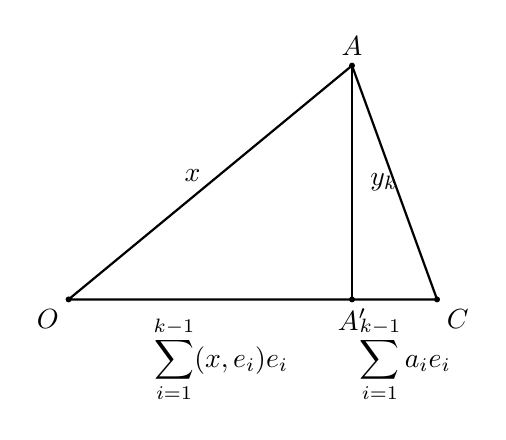
\begin{tikzpicture}[scale=0.9]
  \coordinate (O) at (0,0);
  \coordinate (C) at (5.2,0);
  \coordinate (A) at (4.0,3.3);
  \coordinate (Ap) at (4.0,0);
  \draw[thick] (O)--(A)--(C)--(O);
  \draw[thick] (A)--(Ap);
  \fill (O) circle (1.2pt) node[below left] {$O$};
  \fill (A) circle (1.2pt) node[above] {$A$};
  \fill (Ap) circle (1.2pt) node[below] {$A' $};
  \fill (C) circle (1.2pt) node[below right] {$C$};
  \node[left] at (2.0,1.75) {$x$};
  \node[right] at (4.12,1.65) {$y_k$};
  \node[below] at (2.15,-0.10) {$\displaystyle \sum_{i=1}^{k-1}(x,e_i)e_i$};
  \node[below] at (4.75,-0.10) {$\displaystyle \sum_{i=1}^{k-1}a_i e_i$};
\end{tikzpicture}
\caption{图6-2-1}
\end{figure}
就是说只有作 $x$ 到子空间 $H_{k-1}$（即图6-2-1上直线 $OC$）的正交投影时，才可以达到最小。上面作的图的含意其实超过简单的示意图。因为在内积空间中毕达哥拉斯定理——即勾股定理是成立的：设有两个向量 $y\perp z$，则
\[
 \|y-z\|^2=(y-z,y-z)=\|y\|^2-(y,z)-(z,y)+\|z\|^2=\|y\|^2+\|z\|^2.
\]
我们把这个结果用于 $\triangle AA'C$，$AA'\perp OC$，实际上，
\[
 AA'=y_k=x-\sum_{i=1}^{k-1}(x,e_i)e_i,
\]
所以
\[
 (y_k,e_j)=(x,e_j)-\sum_{i=1}^{k-1}(x,e_i)(e_i,e_j)
 =(x,e_j)-\sum_{i=1}^{k-1}(x,e_i)\delta_{ij}=0,
\]
这里 $j=1,2,\ldots,k-1$。$OC$ 代表 $\{e_1,\ldots,e_{k-1}\}$ 所张的子空间 $H_{k-1}$。$AA'$ 既正交于这空间基底中的一切向量，自然也正交于整个子空间，从而也正交于其一切向量，特别也就正交于
\[
 A'C=\sum_{i=1}^{k-1}(a_i-(x,e_i))e_i.
\]
故由勾股定理有
\[
 |AC|^2=|AA'|^2+|A'C|^2.
\]
但\footnote{校勘：原式在展开内积的一行保留了 $\delta_{ij}$，而指标 $j$ 在该式中游离。利用 $(e_i,e_j)=\delta_{ij}$ 对双重求和收缩后，应直接得到 $\sum_{i=1}^{k-1}|(x,e_i)|^2$，故按此改正。}
\[
 |AC|^2=\left\|x-\sum_{i=1}^{k-1}a_i e_i\right\|^2,
\]
\[
 \begin{aligned}
 |AA'|^2=|OA|^2-|OA'|^2
 &=\|x\|^2-\left\|\sum_{i=1}^{k-1}(x,e_i)e_i\right\|^2\\
 &=\|x\|^2-
 \left(\sum_{i=1}^{k-1}(x,e_i)e_i,
       \sum_{j=1}^{k-1}(x,e_j)e_j\right)\\
 &=\|x\|^2-\sum_{i=1}^{k-1}|(x,e_i)|^2.
 \end{aligned}
\]
\begin{equation}
 |A'C|^2=\sum_{i=1}^{k-1}\|(a_i-(x,e_i))e_i\|^2
 =\sum_{i=1}^{k-1}|a_i-(x,e_i)|^2.
 \tag{20}
\end{equation}
所以只有当 $A'$ 与 $C$ 重合，即 $AC\perp OC$ 时，$|A'C|=0$，这时 $AC$ 才达到最小。即是说当 $a_i=(x,e_i)$ 时，
\[
 \left\|x-\sum_{i=1}^{k-1}a_i e_i\right\|\to\min.
\]

如果(18)式成立，亦即(19)式成立，注意到 $S_N$ 就是这里的 $\sum a_i e_i$，就是此图上的 $OC$，因此(19)式左方之差即这里的 $|AC|^2$。如果(19)式能成立，必有 $|AA'|^2\to0$，就是说，向量 $x$ 的投影当 $k\to\infty$ 时，与原向量之“缺口 $AA'$”会封闭起来。这样我们就会得到判别一个 o.n. 系 $\{e_1,\ldots,e_N,\ldots\}$ 是否 $H$ 的基底的几何方法。

仿照上面的几何方法来计算，我们有

\noindent\textbf{定理10（贝塞尔不等式与帕塞瓦尔等式）}\quad
设 $H$ 为一可分的希尔伯特空间，$\{e_1,\ldots,e_N,\ldots\}$ 是其中的一个 o.n. 系（我们也容许此系只包含有限多个向量的特殊情况），对任一向量 $x$，必有贝塞尔不等式(Bessel inequality)
\begin{equation}
 \sum_{i=1}^\infty |(x,e_i)|^2\le\|x\|^2,
 \tag{21}
\end{equation}
成立。o.n. 系 $\{e_1,\ldots,e_N,\ldots\}$ 是 $H$ 的基底的充分必要条件是上式变成等式，称为帕塞瓦尔等式(Parseval's identity)或称封闭性方程式：
\begin{equation}
 \sum_{i=1}^\infty |(x,e_i)|^2=\|x\|^2.
 \tag{22}
\end{equation}
这时，我们说 $\{e_1,\ldots,e_N,\ldots\}$ 是一个完全的 o.n. 系。

\noindent\textbf{证}\quad
令 $x_i=(x,e_i)$，则仿照上面的证明有
\[
 \left\|x-\sum_{i=1}^{k-1}x_i e_i\right\|^2
 =\|x\|^2-\sum_{i=1}^{k-1}|x_i|^2.
\]
因为上式左方非负，故有
\[
 \sum_{i=1}^{k-1}|x_i|^2\le\|x\|^2.
\]
令 $k\to\infty$ 即得(21)式。

再证帕塞瓦尔等式的必要性，若 $\{e_1,\ldots,e_N,\ldots\}$ 是 $H$ 之基底，则一定存在一列复数 $c_i$，使
\[
 \left\|x-\sum_{i=1}^N c_i e_i\right\|\to0.
\]
令 $x_i=(x,e_i)$，仿上面的作法有\footnote{校勘：原式中间一项写作 $\left\|\sum_{i=1}^{k-1}x_i e_i\right\|^2$，但本段固定的部分和指标为 $N$，上下文及下一行均要求上限为 $N$，故改正。}
\[
 \begin{aligned}
 \left\|x-\sum_{i=1}^N c_i e_i\right\|^2
 &=\|x\|^2-
 \left\|\sum_{i=1}^{N}x_i e_i\right\|^2
 +\sum_{i=1}^N|x_i-c_i|^2\\
 &\ge\|x\|^2-\sum_{i=1}^N|x_i|^2\ge0
 \qquad(\text{贝塞尔不等式}).
 \end{aligned}
\]
若左方当 $N\to\infty$ 时趋于0，自然有帕塞瓦尔等式成立。

充分性证明如下。若(22)成立，则
\[
 \lim_{N\to\infty}\left\|x-\sum_{i=1}^N x_i e_i\right\|\to0,
\]
这就是说，一定能找到复数 $c_i$，使
\[
 \left\|x-\sum_{i=1}^N c_i e_i\right\|^2\to0
\]
（取 $c_i=(x,e_i)$ 即可），所以 $\{e_1,\ldots,e_N,\ldots\}$ 是基底。证毕。

希尔伯特空间 $H$ 中的 o.n. 系 $\{e_1,\ldots,e_N,\ldots\}$ 是一个基底，也就是说它是一个完全的 o.n. 系，还有另一个几何解释，即如果 $\{e_1,\ldots,e_N,\ldots\}$ 是 $H$ 中的一个完全的 o.n. 系，则不可能再找到一个非0的 $e\in H$，使 $e\perp e_i,i=1,2,\ldots,N,\ldots$。事实上，若有 $e\in H,\|e\|=1$，而且 $e\perp e_i,i=1,2,\ldots$，则对 $e$ 应用(22)式当有
\[
 \|e\|^2=\sum_{i=1}^\infty |(e,e_i)|^2=0,
\]
这与 $\|e\|=1$ 矛盾。上面的论断之逆也是对的，即是说：如果 $\{e_1,\ldots,e_N,\ldots\}$ 不是 $H$ 中完全的 o.n. 系，则一定有一个 $x\in H$，使(21)成为严格的不等式：
\[
 \sum_{i=1}^\infty |(x,e_i)|^2<\|x\|^2.
\]
但若令
\[
 y=\sum_{i=1}^\infty(x,e_i)e_i,
\]
这个级数在范数意义下是收敛的。因为考虑 $\sum_{i=1}^\infty(x,e_i)e_i$ 之两个部分和 $S_{N_1}$ 与 $S_{N_2}$，$N_2>N_1$，则容易证明，
\[
 \|S_{N_2}-S_{N_1}\|^2=\sum_{i=N_1+1}^{N_2}|(x,e_i)|^2.
\]
由贝塞尔不等式，上式右方当 $N_1$ 和 $N_2\to\infty$ 时必趋于0，所以 $\{S_N\}$ 是 $H$ 中的柯西序列，因此有一个 $y\in H$ 使
\[
 y=\sum_{i=1}^\infty(x,e_i)e_i.
\]
显然
\[
 \|y\|^2=\lim_{N\to\infty}(S_N,S_N)=\sum_{i=1}^\infty|(x,e_i)|^2.
\]
于是 $y\ne x$，因为由 $\{e_1,\ldots,e_N,\ldots\}$ 不完全的假设我们已知上式右方 $<\|x\|^2$。但是我们可以证明 $(y,e_i)=(x,e_i)$。事实上，若 $N$ 充分大（$N>i$），$(S_N,e_i)=\sum_{j=1}^N(x,e_j)(e_j,e_i)=\sum_{j=1}^N(x,e_j)\delta_{ji}=(x,e_i)$，所以
\[
 (y,e_i)=(y-S_N,e_i)+(S_N,e_i)=(y-S_N,e_i)+(x,e_i).
\]
但是 $|(y-S_N,e_i)|\le\|y-S_N\|\,\|e_i\|=\|y-S_N\|\to0$。所以 $(y,e_i)=(x,e_i)$ 对一切 $i$ 成立。即是说 $(x-y)\perp e_i$，对一切 $i$ 成立。令 $e=x-y$，我们找到了 $H$ 中的一个非0的、正交于一切 $e_i$ 的元 $e$。

现在再回到 $L^2$ 空间。第四章中，我们着重指出，对于两个 $L^2([0,2\pi])$ 函数 $f(x)$ 与 $g(x)$，定义
\begin{equation}
 (f,g)=\int_0^{2\pi}f(x)\overline{g(x)}\,dx
 \tag{23}
\end{equation}
成为一个内积。在这样的内积下，$L^2([0,2\pi])$ 是一个复内积空间。

而且因为 $L^2([0,2\pi])$ 是一个完备空间（里斯--费希尔定理），所以这是一个希尔伯特空间。它是一个可分希尔伯特空间，因为它具有一个完全的 o.n. 系
\[
 \left\{\frac1{\sqrt{2\pi}}e^{inx}\right\},\qquad n=0,\pm1,\pm2,\ldots.
\]
对于其中的任一元 $f$，
\[
 (f,e_n)=\frac1{\sqrt{2\pi}}\int_0^{2\pi}f(x)e^{-inx}\,dx.
\]

除了相差一个常数因子外就是 $f(x)$ 的傅里叶系数，而对 $L^2([0,2\pi])$ 函数，公式
\[
 \int_0^{2\pi}|f(x)|^2\,dx=\sum_{n=0,\pm1,\ldots}|(f,e_n)|^2
\]
是已经证明了的。

重要的事实是，$L^2([0,2\pi])$ 是一个“典型的”可分希尔伯特空间。事实上，任给一个可分希尔伯特空间 $H$，定理9告诉我们，它一定具有一个完全的 o.n. 系 $\{e_i\},i=0,\pm1,\ldots,\pm n,\ldots$。这里我们对其指标 $i$ 重新作了编号，使它可取一切正、负整数值。我们现在在 $H$ 与 $L^2([0,2\pi])$ 中建立如下的一一对应：对于 $\widetilde f\in H$，我们可以作函数
\[
 f(x)=\sum_j f_j\frac1{\sqrt{2\pi}}e^{ijx}
\]
与 $\widetilde f$ 相对应。这里 $f_j=(\widetilde f,e_j)$。这个函数确实是存在的，因为
\begin{equation}
 \widetilde f=\sum_j f_j e_j.
 \tag{24}
\end{equation}
而由于 $H$ 是一个希尔伯特空间，由(21)式，$\sum_j|f_j|^2<+\infty$。因此这个级数在 $L^2([0,2\pi])$ 中收敛。所以可以记其和为 $f(x),f\in L^2([0,2\pi])$，而且
\[
 f_j=\int_0^{2\pi}f(x)\frac1{\sqrt{2\pi}}e^{-ijx}\,dx.
\]
反之，若有一个 $f(x)\in L^2([0,2\pi])$，则可用上式作其傅里叶系数 $f_j$，而用(24)式作一个 $\widetilde f$，很容易证明 $\widetilde f\in H$。总之，$L^2([0,2\pi])$ 与 $H$ 有一个保持线性关系的同构。在这个同构关系下，内积和范数都不变：设有另一个 $\widetilde g\in H$，对应于另一个 $g(x)\in L^2([0,2\pi])$，它们的傅里叶系数是
\[
 g_j=(\widetilde g,e_j)=\int_0^{2\pi}g(x)\frac1{\sqrt{2\pi}}e^{-ijx}\,dx,
\]
则由帕塞瓦尔等式有
\[
 \|f\|^2=\sum_j|f_j|^2=\|\widetilde f\|_H^2,
\]
\[
 (f,g)_{L^2}=\sum_j f_j\overline{g_j}=(\widetilde f,\widetilde g)_H.
\]
所以这种对应保持内积与范数均不变。总之是等距同构。希尔伯特空间除了有线性结构以外，就只有内积与范数，决定了其所有性质。在这个意义下，所有的可分希尔伯特空间，本质上都是 $L^2([0,2\pi])$。

关于度量空间以及赋范线性空间我们就讲到这里为止。度量空间的另一些性质如紧性与连通性就都移到下节去讨论。这一方面是由于本节篇幅太长，同时也只讨论度量空间，而紧性与连通性在一般的拓扑空间中讨论更合适，所以宁可在下一节讲。在那里可以更清楚地看到，度量空间中的紧性与一般拓扑空间中的紧性有什么区别。
